% !TEX root = memoria-tfg/memoria.tex

\documentclass[oneside,a4paper,12pt]{book} % TODO: cambia "oneside" por "twoside" a la hora de imprimirlo

\usepackage[spanish]{babel}
\usepackage[utf8]{inputenc}
\usepackage{geometry}
\usepackage{makeidx}
\usepackage[hyphens]{url}
\usepackage{graphicx}
\usepackage{color}
\usepackage{caption}
\usepackage{acronym}
\usepackage{hyphenat}
\usepackage{a4wide}
\usepackage[normalsize]{subfigure}
\usepackage{float}
\usepackage{titlesec}
\usepackage[Lenny]{fncychap}
\usepackage{listings}
\usepackage{eurosym} % para poder usar el símbolo del euro con \euro {xx}
\usepackage{hyperref} % TODO: añade la opción hidelinks para imprimirlo (los enlaces no aparecerán resaltados)
\usepackage{xcolor}
\usepackage{tabularx}
\usepackage[hyphenbreaks]{breakurl}
\usepackage{multicol}
\usepackage{amsmath}
\usepackage{parskip}
\usepackage[bottom]{footmisc} % Paquete para personalizar encabezados y pies de página
\usepackage{appendix}


\setlength{\parskip}{1em}
\setlength{\parindent}{1cm}

\renewcommand{\thefootnote}{\arabic{footnote}} % Opcional: para cambiar el formato de los números de los pies de página

\usepackage[square,numbers]{natbib}
\AtBeginDocument{
  \renewcommand{\bibsection}{\chapter{\bibname}}
} % Bibliografia en capitulo numerado

\colorlet{punct}{red!60!black}
\definecolor{background}{HTML}{EEEEEE}
\definecolor{delim}{RGB}{20,105,176}
\colorlet{numb}{magenta!60!black}

% Para que no parta las palabras
\pretolerance=10000

\newcommand{\bigrule}{\titlerule[0.5mm]} \titleformat{\chapter}[display] % cambiamos el formato de los capítulos
{\bfseries\Huge} % por defecto se usaron caracteres de tamaño huge en negrita
{% contenido de la etiqueta 
\titlerule % línea horizontal 
\filright % texto alineado a la derecha 
\Large\chaptertitlename\ % capítulo e índice en tamaño large
\Large % en lugar de 
\Huge \Large\thechapter} 
{0mm} % espacio mínimo entre etiqueta y cuerpo
{\filright} % texto del cuerpo alineado a la derecha
[\vspace{0.5mm} \bigrule] % después del cuerpo, dejar espacio vertical y trazar línea horizontal gruesa
\titlespacing*{\chapter}{0pt}{5pt}{20pt} % Espacios alrededor del título del capítulo
\geometry{a4paper, left=2.5cm, right=2.5cm, top=2.5cm, bottom=2.0cm, headsep=1.0cm}


% Estilos para ilustrar códigos:
\definecolor{code_green}{rgb}{0,0.6,0}
\definecolor{code_gray}{rgb}{0.5,0.5,0.5}
\definecolor{code_mauve}{rgb}{0.58,0,0.82}

\lstset{frame=tb,
  language=C,
  aboveskip=3mm,
  belowskip=3mm,
  showstringspaces=false,
  columns=flexible,
  basicstyle={\small\ttfamily},
  numbers=none,
  numberstyle=\tiny\color{code_gray},
  keywordstyle=\color{blue},
  commentstyle=\color{code_green},
  stringstyle=\color{code_mauve},
  breaklines=true,
  breakatwhitespace=true,
  tabsize=3
}

\lstset{frame=tb,
  language=C++,
  aboveskip=3mm,
  belowskip=3mm,
  showstringspaces=false,
  columns=flexible,
  basicstyle={\small\ttfamily},
  numbers=none,
  numberstyle=\tiny\color{code_gray},
  keywordstyle=\color{blue},
  commentstyle=\color{code_green},
  stringstyle=\color{code_mauve},
  breaklines=true,
  breakatwhitespace=true,
  tabsize=3
}

\lstset{frame=tb,
  language=Python,
  aboveskip=3mm,
  belowskip=3mm,
  showstringspaces=false,
  columns=flexible,
  basicstyle={\small\ttfamily},
  numbers=none,
  numberstyle=\tiny\color{code_gray},
  keywordstyle=\color{blue},
  commentstyle=\color{code_green},
  stringstyle=\color{code_mauve},
  breaklines=true,
  breakatwhitespace=true,
  tabsize=3
}

\lstdefinelanguage{json}{
    basicstyle=\normalfont\ttfamily,
    numbers=left,
    numberstyle=\scriptsize,
    stepnumber=1,
    numbersep=8pt,
    showstringspaces=false,
    breaklines=true,
    frame=lines,
    backgroundcolor=\color{background},
    literate=
     *{0}{{{\color{numb}0}}}{1}
      {1}{{{\color{numb}1}}}{1}
      {2}{{{\color{numb}2}}}{1}
      {3}{{{\color{numb}3}}}{1}
      {4}{{{\color{numb}4}}}{1}
      {5}{{{\color{numb}5}}}{1}
      {6}{{{\color{numb}6}}}{1}
      {7}{{{\color{numb}7}}}{1}
      {8}{{{\color{numb}8}}}{1}
      {9}{{{\color{numb}9}}}{1}
      {:}{{{\color{punct}{:}}}}{1}
      {,}{{{\color{punct}{,}}}}{1}
      {\{}{{{\color{delim}{\{}}}}{1}
      {\}}{{{\color{delim}{\}}}}}{1}
      {[}{{{\color{delim}{[}}}}{1}
      {]}{{{\color{delim}{]}}}}{1},
}

% Definición de mis propios tipos: Códigos, Ecuaciones y Tablas
\DeclareCaptionType{code}[Código][Listado de códigos]
\DeclareCaptionType{myequation}[Ecuación][Listado de ecuaciones]

% TODO: especifica las reglas de separación que consideres. Algunos ejemplos:
\hyphenation{fuer-tes}
\hyphenation{mul-ti-ca-pa}
\hyphenation{res-pues-ta}
\hyphenation{di-fe-ren-tes}
\hyphenation{de-sa-rro-lla-dos}
\hyphenation{re-pre-sen-tan-do}

 % archivo de configuraci�n de estilo

\makeindex

\begin{document}
\baselineskip 1.35\baselineskip

\frontmatter

\thispagestyle{empty}
\vspace{2cm}

\begin{figure}[htb]
  \centerline{\resizebox{.60\textwidth}{!}{
\includegraphics{figs/logo_urjc}}}
\end{figure}

\begin{center}
  {\Large {\bf GRADO EN INGENIERÍA DE ROBÓTICA SOFTWARE}}
  \vspace{5mm}
 
  {\large {Escuela de Ingeniería de Fuenlabrada}}
  \vspace{5mm}

  {\large {Curso académico 2023-2024}}

  \vspace{1cm}

  {\large {\bf Trabajo Fin de Grado}}

  \vspace{2cm}

  {\Large {Navegación Autónoma de drones basado en\\
          inteligencia artificial y aprendizaje por refuerzo\\[1cm] }}

  \vspace{5cm}
  {\bf Autor}: Bárbara Villalba Herreros \\
  {\bf Tutor}: Dr. Roberto Calvo Palomino 

\end{center}

\clearpage
\thispagestyle{empty}


% Este diseño se corresponde con la licencia CC-BY-NC-SA.
% Por supuesto, puedes poner la licencia que mejor se adapte al propósito de tu trabajo.
% Recuerda que, si no se especifica ninguna licencia, esta -como cualquier creación artística- pasaría a estar licenciada con todos los derechos reservados (copyright).

\cleardoublepage

\begin{figure}
 \ \ \ \ 
\includegraphics[width=0.25\linewidth]{figs/by-nc-sa.png}
 \label{fig:cc} 
 \end{figure}

\

\

\

\noindent
Este trabajo se distribuye bajo los términos de la licencia internacional \href{http://creativecommons.org/licenses/by-nc-sa/4.0/}{CC BY-NC-SA International License} (Creative Commons AttributionNonCommercial-ShareAlike 4.0). Usted es libre de \textit{(a) compartir}: copiar y redistribuir el material en cualquier medio o formato; y \textit{(b) adaptar}: remezclar, transformar y crear a partir del material. El licenciador no puede revocar estas libertades mientras cumpla con los términos de la licencia:

\begin{itemize}
\item \textit{Atribución}. Usted debe dar crédito de manera adecuada, brindar un enlace a la licencia, e indicar si se han realizado cambios. Puede hacerlo en cualquier forma razonable, pero no de forma tal que sugiera que usted o su uso tienen el apoyo de la licenciante.
\item \textit{No comercial}. Usted no puede hacer uso del material con propósitos comerciales.
\item \textit{Compartir igual}. Si remezcla, transforma o crea a partir del material, debe distribuir su contribución bajo la la misma licencia del original.
\end{itemize}

\begin{flushright}
		\vspace{7.0 cm}
		\emph{Documento de} \textbf{Bárbara Villalba}. % TODO: pon aquí tu nombre cuando hagas el documento
\end{flushright}



\cleardoublepage

\chapter*{Agradecimientos}

En primer lugar queria agradecer a todas las personas que han sido parte de este camino y trayectoria, agradezco a mis tres familias por apoyarme y no 
dejarme rendirme en ningún momento. Agradeciendo así a la madre de mi pareja por estar escuchandome tendida y aconsejando me. \newline
\newline
Mención especial a mi pareja Renato Luigi por estar a pie de cañón en todo momento ayudando, apoyando, y escuchando, no me olvidaré de las charlas que teníamos
en el coche mientras cenabamos. También queria agradecer a mi padre por sus charlas telefónicas de vuelta a casa, en donde me intentaba ayudar con sus ideas. Además de mi madre,
mi hermana y abuelos por estar siempre a mi lado.\newline
\newline
En segundo lugar, quiero mencionar a mi cuñado Angelo Vincenzo por ser compañero de carrera y poder haber compartido una variedad de recuerdos que nunca olvidaré. \newline
\newline
Además de agradecer a mi tutor Roberto por la paciencia que ha tenido durante el desarrollo de este trabajo y brindarme ánimos en el camino. \newline
\newline
Finalmente, dar las gracias a las personas que no pueden estar en estos momentos.


\begin{flushright}
	\vspace{4.0 cm}
	\emph{A alguien especial,\\
    que esta en el cielo, Vincenzo Barra.}\\
	\emph{Bárbara Villalba}
\end{flushright}

\thispagestyle{empty}



\cleardoublepage

\chapter*{Resumen\markboth{Resumen}{Resumen}}

Una de las principales áreas de estudio de la robótica es la navegación autónoma. En la actualidad, ésta se lleva a cabo mediante dos tipos de 
algoritmos, enfoques clásicos que se 
basan en la planificación de rutas y trayectorias mediante algoritmos que conocen el mapa del escenario, o cada vez tomando más protagonismo aquellos basados 
en Inteligencia Artificial (IA), que consisten en aprender y adaptarse a escenarios. Dentro de la robótica aérea se están 
creando una gran número de aplicaciones variadas gracias a la capacidad de los drones, que ofrecen una perspectiva diferente del 
entorno y alcanzan zonas en los que un robot con ruedas o humanos no podrían llegar.

En este TFG se explora un método de navegación basado en IA y aprendizaje por refuerzo, 
cuyo objetivo es que el dron navegue en un área determinada, en este caso un carril de una carretera.
Este tipo de navegación, tiene muchas aplicaciones, por ejemplo, la inspección de carreteras a gran altura para analizar el estado de las mismas, tráfico, 
accidentes, primeros auxilios en desastres climatológicas.

Este trabajo propone el uso de técnicas de IA utilizando Deep Learning, como las redes neuronales de segmentación para la detección del carril y extracción 
de sus características. Así como algoritmos de aprendizaje por refuerzo, en este caso, Q-learning, para que el sistema de control del 
dron sea capaz de aprender las acciones a realizar en función de la información sensorial obtenida y sea capaz de generalizar.

Todo ello se ha realizado empleando el simulador AirSim, en el que se simula un entorno foto-realista, donde el dron realiza un seguimiento del carril. Por último, se emplea el middleware robótico ROS
para las comunicaciones entre el simulador, y el software implementado en esta solución.


\cleardoublepage

\chapter*{Acrónimos\markboth{Acrónimos}{Acrónimos}}

% Añade a continuación los acrónimos que uses en el documento. Algunos ejemplos:
\begin{acronym}
	\acro{UAV}{\emph{Unmanned Air Vehicle}}
	\acro{UAS}{\emph{Unmanned Air System}}
	\acro{GCS}{\emph{Ground Control Station}}
	\acro{IA}{\emph{Inteligencia Artificial}}
	\acro{Airsim}{\emph{Aerial Informatics and Robotics Simulation}}
	\acro{AGV}{\emph{Automated Guided Vehicles}}
	\acro{AMR}{\emph{Autonomous Mobile Robots}}
	\acro{TFG}{\emph{Trabajo de fin de Grado}}
	\acro{ROS}{\emph{Robotic Operative System}}
	\acro{Mavros}{\emph{MAVlink to ROS Interface}}
	\acro{ML}{\emph{Machine Learning}}
	\acro{API}{\emph{Application programming interface}}




\end{acronym}


\cleardoublepage

\tableofcontents

\listoffigures

\listofcodes

\listofmyequations

\listoftables

%\pagestyle{empty}

\cleardoublepage

 % aqui se cargan todas las "primeras paginas"

% Bibliografia
\let\OLDthebibliography=\thebibliography
\def\thebibliography#1{\OLDthebibliography{#1}
\addcontentsline{toc}{chapter}{\bibname}}

\mainmatter

\setcounter{page}{1}

\chapter{Introducción}
\label{cap:introduccion}
\setcounter{page}{1}

La evolución tecnológica ha provocado una transformación radical en nuestra forma de vivir, trabajar y relacionarnos desempeñando la tecnología un papel 
fundamental en el avance de la sociedad e impulsando una serie de innovaciones que se extienden desde la invención de la rueda hasta la era digital contemporánea. 
Por ejemplo, los ordenadores empezaron siendo grandes máquinas que ocupaban habitaciones enteras que requerían una gran cantidad de energía y mantenimiento. Hoy en día, los ordenadores
son dispositivos ligeros y eficientes que pueden realizar múltiples cálculos por segundos que se utilizan en diferentes ramas de las ingenierías como la informática, telecomunicaciones y,
por supuesto, la robótica. \newline

La robótica, en particular, se destaca como una de las ramas de la tecnología que más impacto significativo ha tenido. Estos avances han facilitado numerosas tareas mejorando la eficiencia 
y la capacidad de enfrentar desafíos complejos dando pie a nuevas posibilidades en nuestro entorno. Un ejemplo de ello puede ser la robótica aérea con el uso de los drones, 
demostrando ser desafiantes y valiosos en la inspección de áreas de difícil acceso, el mapeo de terrenos, la realización de entregas, la navegación autónoma o la captura 
de imágenes desde alturas elevadas. Su versatilidad y su capacidad para poder operar en entornos peligrosos o inaccesibles para los seres humanos los convierten 
en herramientas fundamentales en campos como la agricultura, la seguridad, la investigación medioambiental y la logística. 

\section{La robótica}
\label{sec:enfoquesrobotica}
Como mencionamos anteriormente, entre las diversas ramas de la tecnología, la robótica se destaca como una de las más prometedoras. Apareciendo como disciplina durante la década de los años 60, 
la robótica ha tenido un cambio asombroso  pasando de ser simples máquinas programables a sistemas inteligentes capaces de aprender y adaptarse 
a su entorno teniendo avances en diversas disciplinas de la ingeniería, como la informática, la inteligencia artificial, la ingeniería de control, la mecánica, 
la electricidad y la electrónica. 
Los robots de hoy en día no solo tienen la capacidad de realizar tareas programadas y repetitivas, sino que también tienen la capacidad de interactuar con su entorno, 
tomar decisiones basadas en la información sensorial y aprender de sus experiencias. Este avance en la robótica nos ha permitido tener una definición más precisa de lo que es 
la robótica moderna, definiendo la robótica como ciencia interdisciplinaria encargada de la creación, funcionamiento, estructuración, fabricación y uso de los robots. 
Esta definición incluye no solo los componentes mecánicos y eléctricos, sino que también los algoritmos de control, los sensores que les permiten recopilar
datos de su entorno y los sistemas que procesan esta información y toman decisiones.

\begin{figure} [H]
  \begin{center}
    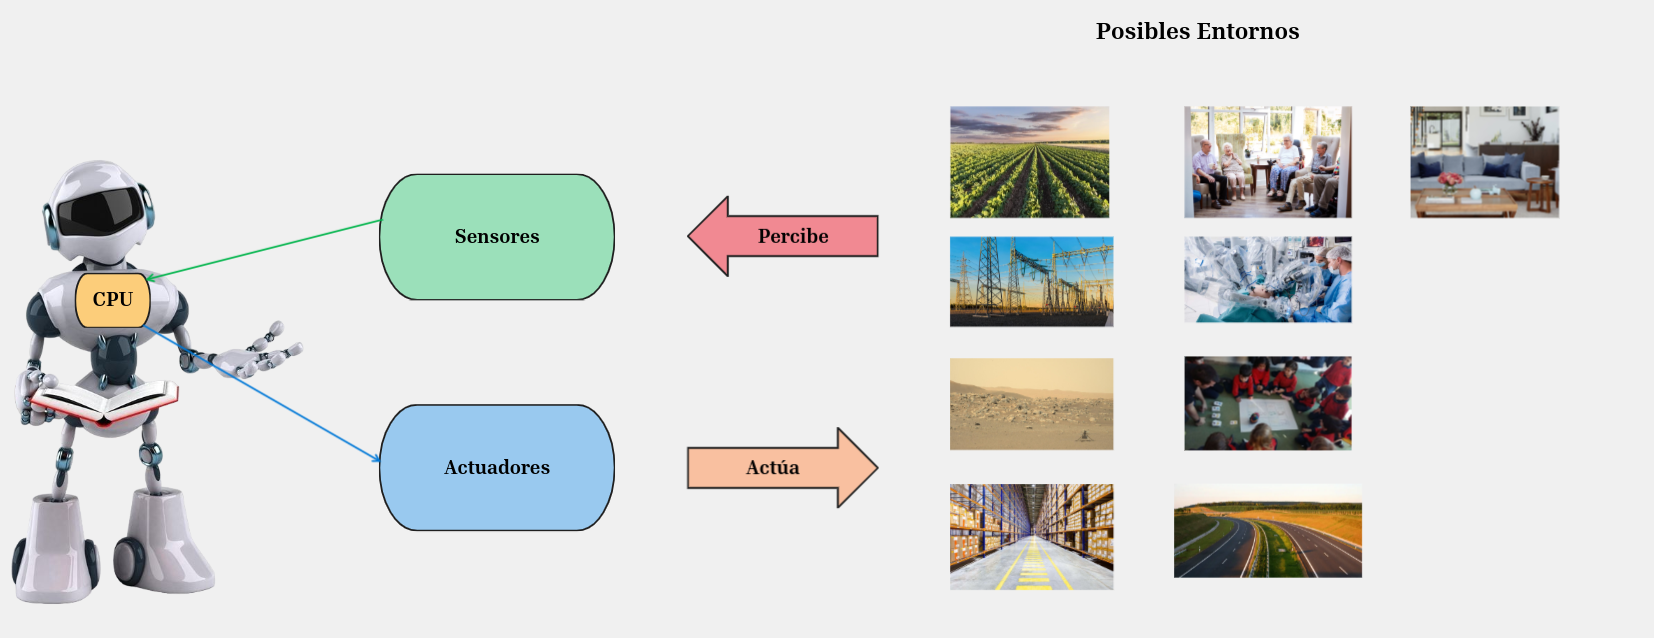
\includegraphics[scale=0.25]{figs/introducción/robot.png}
  \end{center}
  \caption{Definición de robot.}
  \label{fig:robot}
\end{figure}\

La capacidad de los robots para aprender y adaptarse a su entorno abre nuevas oportunidades en campos como la medicina, la exploración lunar, la asistencia personal, la automatización industrial, etc. 
Además de abrir nuevas aplicaciones y tareas como puede ser la navegación autónoma, la detección de objetos o 
la manipulación de objetos con sensores táctiles y de fuerza, dichas tareas que pueden realizar, pueden ser peligrosas, delicadas, sucias o monótonas 
(conocidas como las 4D's: dull,dirty, dangerous and dear)\footnote{\url{https://www.forbes.com/sites/bernardmarr/2017/10/16/the-4-ds-of-robotization-dull-dirty-dangerous-and-dear/?sh=40bb6cec3e0d}}


 % etiqueta para luego referenciar esta sección
 \subsection{Enfoques de control en el mundo de la robótica}
 \label{sec:enfoquesrobotica}
A lo largo de la evolución de la robótica, han surgido tres enfoques fundamentales para el diseño y la operación de robots. Cada uno de estos enfoques presentan diferentes
formas de interactuar y operar robots, con sus riesgos, características y aplicaciones únicas. 

\subsubsection{Teleoperación}
\label{sec:subseccion}

La teleoperación surge de la necesidad de manipular objetos o realizar tareas en entornos complejos, peligrosos y distantes para el ser humano. Desde la historia, el ser humano
ha utilizado una variedad de herramientas para ampliar su capacidad de manipulación como palos utilizados para caer la fruta madura de un árbol. Con el tiempo, se desarrollaron 
dispositivos más complejos, como pinzas que permitían manipular piezas o alcanzar objetos de difícil acceso facilitando el trabajo para el operario. En la era moderna, la teleoperación
ha estado evolucionando hasta el punto de incluir sistemas robóticos robustos que pueden ser controlados a distancia, permitiendo al operario poder realizar
tareas en entornos peligrosos e inaccesibles para el ser humano como puede ser la exploración espacial, la medicina o la inspección nuclear.
La intervención del operador humano en los sistemas de teleoperación de robots es imprescindible, debe ser capaz de poder interpretar los datos sensoriales que proporciona el robot, así como de 
tomar decisiones robustas y precisas dependiendo de la situación. Esto conlleva tener una capacidad de realizar múltiple tareas simultáneamente adpatandose a situaciones imprevistas. \newline

Hoy en día, la teleoperación de robots tiene variedad de aplicaciones. Una de ellas puede ser la exploración espacial, en donde se utiliza la teleoperación
como técnica de manipulación remota como el Sojourner Rover. Como se muestra en la figura \ref{fig:Sojourner}, El Sojourner Rover\footnote{\url{https://www.astronomy.com/space-exploration/sojourner-nasas-first-mars-rover/}} 
es un pequeño robot móvil compuesto por 6 ruedas creado por los científicos de la NASA para estudiar 
la superficie de Marte con la capacidad de enviar imágenes en directo y realizar análisis del terreno del planeta. Gracias a sus ruedas podía moverse por terrenos rocosos y de difícil acceso
ya que estaban equipadas materiales como de aluminio y acero inoxidable. \newline

\begin{figure} [H]
  \begin{center}
    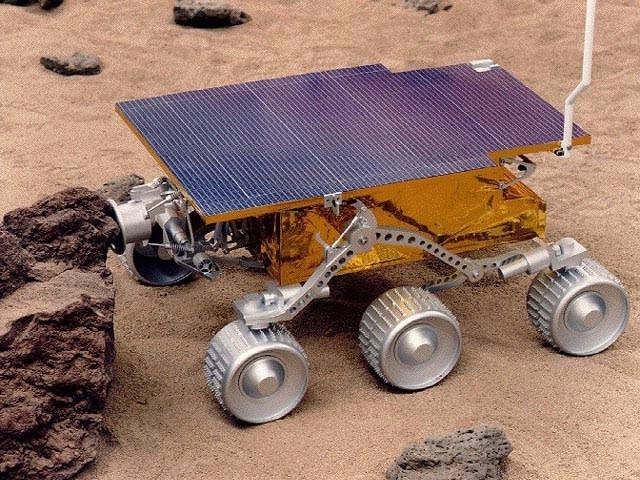
\includegraphics[scale=0.4]{figs/introducción/Sojourner.jpg}
  \end{center}
  \caption{Sojourner Rover}
  \label{fig:Sojourner}
\end{figure}\

Con esta misión espacial se pudo probar como era el entorno marciano con técnicas realizadas en los laboratorios de la NASA demostrando que se podía realizar una teleoperación en 
el espacio abriendo el camino a futuros rovers como el Spirit, Opportunity y más\footnote{\url{https://spaceplace.nasa.gov/mars-spirit-opportunity/sp/}}. \newline

A pesar de ser un buen enfoque en cuanto a controlar un robot, presenta sus propias limitaciones, como la dependencia de una conexión continua y confiable entre
el operario y el robot. Si la conexión se interrumpe, el control del robot podría perderse desembocando situaciones de grave peligro. Otro tipo de limitación puede ser la carga
cognitiva que puede tener el operario al controlar el robot, ya que el operario debe permanecer concentrado monitorizando y controlando el robot de manera constante.
Lo último puede conducir a errores humanos, especialmente durante operaciones de larga duración, lo que hace interesante tener otro tipo de enfoque de control.

\subsubsection{Robótica Semiautónoma}
\label{sec:subseccion}
Los robots pueden realizar tareas de forma independiente siguiendo instrucciones preprogramadas o tomando decisiones en tiempo real, este enfoque se le conoce como autonomía o semi-autonomía, 
siendo la diferencia que en el enfoque semi-autónomo todavía existe parte de teleoperación en el robot. Este enfoque permite que los robots puedan ser autónomos para poder
percibir su entorno y en la toma de decisiones, pero con el handicap de que un operario humano pueda controlarlo para poder ajustar parámetros, cambiar objetivos o intervenir 
en caso de emergencia. \newline

Aunque los robots semi-autónomos puedan tomar decisiones en tiempo real, a menudo siguen instrucciones preprogramadas o reciben ordenes de un operario humano, esta toma de decisiones
puede incluir elegir la ruta más eficiente para navegar por un entorno peligroso como puede ser el robot submarino llamado Nereus como se ilustra en la figura \ref{fig:Nereus}. El Nereus\footnote{\url{https://www.bbc.com/mundo/ciencia_tecnologia/2009/06/090603_1541_nereus_robot_mar_mr}} 
es un vehículo submarino semi-autónomo que puede ser manejado por control remoto que entro en servicio en el año 2009, su propósito fue explorar la Fosa de las Marianas, específicamente el Abismo Challenger (es el punto más
profundo conocido en los océanos). Fue manejado mediante control remoto por pilotos que se encontraban en un barco en la superficie, aunque el Nereus también podía cambiar al modo
de vehículo autónomo pudiendo navegar libremente adaptándose a las condiciones del entorno sin intervención humana directa. \newline

\begin{figure} [H]
  \begin{center}
    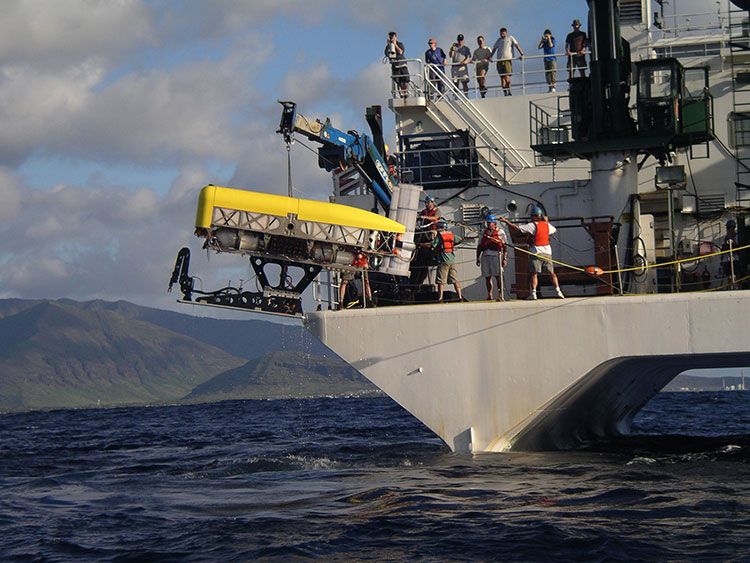
\includegraphics[scale=0.4]{figs/introducción/nereus.jpg}
  \end{center}
  \caption{Nereus}
  \label{fig:Nereus}
\end{figure}\

Lamentablemente, en 2014 durante una misión, el robot Nereus sufrió un colapso estructural y se perdió en el fondo del océano. A pesar de esta perdida, los datos que se pudieron
recopilar en este robot submarino siguen siendo una fuente de conocimiento sobre las profundidades marinas. Este ejemplo de robot semi-autónomo demuestra que se pueden realizar 
tareas en entornos peligrosos sin poner en riesgo la vida humana aunque tenga control por un operario\footnote{\url{https://www.elperiodico.com/es/ciencia/20140512/famoso-sumergible-nereus-pierde-fondo-mar-3271389}}. 

En cuanto a las debilidades de la robótica semiautonóma, estos robots 
aún requieren intervención humana para tareas complejas o situaciones imprevistas, aunque la dependencia del operario sea menor todavía sigue siendo significativa. 
Se debe garantizar la seguridad y la fiabilidad de estos sistemas semi-autónomos, cualquier fallo en la autonomía del robot 
o en la intervención humana puede tener consecuencias peligrosas y asimismo de que los algoritmos perceptivos y de control de los robots semi-autónomos deben ser eficientes y 
robustos ante situaciones cambiantes.

\subsubsection{Robótica Autónoma}
\label{sec:subseccion}

La robótica autónoma consiste en desarrollar robots que sean capaces de operar y realizar tareas de forma independiente sin la intervención de un ser humano. En contraste con los 
robots teleoperados, este tipo de robots necesitan un comportamiento más robusto y preciso para realizar tareas independientes basándose en la percepción del entorno 
y en la toma de decisiones autónomas.
El concepto de automía en los sistemas robóticos se esta convirtiendo en un área de investigación activa y en rápido desarrollo. Los avances en inteligencia artificial (IA), visión 
artificial, aprendizaje automático han facilitado la creación de robots autónomos capaces de llevar a acabo amplias variedades de tareas en entornos no estructurados y cambiantes. 
Uno de los grandes desafíos que enfrenta la robótica autónoma es cómo el robot puede realizar la percepción del entorno, identificando y comprendiendo objetos y situaciones de manera
precisa y en tiempo real. \newline

Por ejemplo, como se muestra en la figura \ref{fig:Rega}, el robot autónomo parecido a un helicóptero diseñado por investigadores suizos es capaz de realizar tareas de 
rescate y búsqueda en los Alpes suizos\footnote{\url{https://www.swissinfo.ch/spa/ciencia/drones-suizos-al-rescate/46203902}}. Este dron autónomo puede llegar a escanear amplias zonas de montaña y reconocer personas en tierra de manera autónoma mediante
cámaras y algoritmos de aprendizaje automático desarrollados por la ETH Zúrich. Facilitando las tareas de rescate al equipo de rescate Rega siguiendo rutas
predefinidas sin intervención humana directa localizando a personas atrapadas o en peligro en áreas remotas o accidentadas.

\begin{figure} [H]
  \begin{center}
    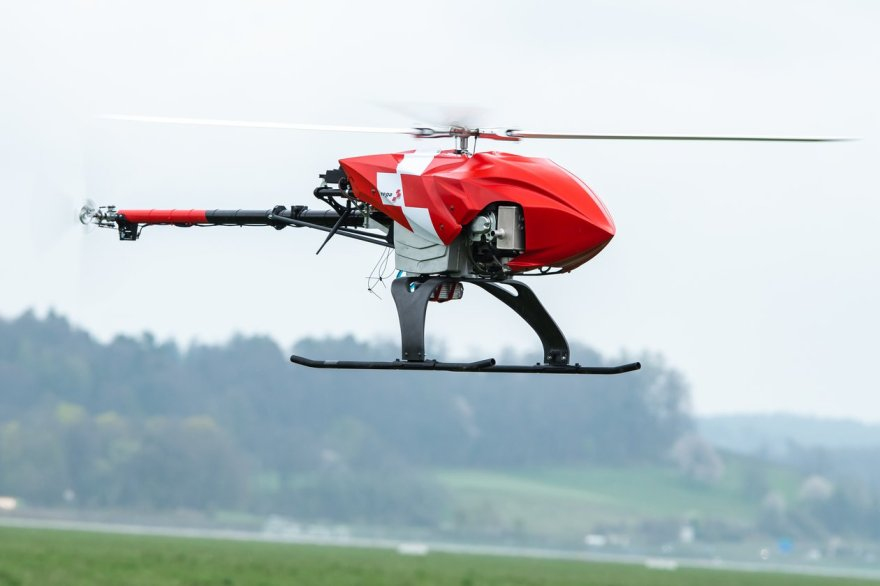
\includegraphics[scale=0.4]{figs/introducción/Rega.jpg}
  \end{center}
  \caption{El dron de rescate Rega}
  \label{fig:Rega}
\end{figure}\

\section{Robótica aérea}
\label{sec:subseccion}

Dentro del campo de la robótica aérea tenemos los drones. Podemos definir un dron, como vehículo aéreo no tripulado (UAV), es un tipo de aeronave que puede operar sin la 
necesidad de un piloto humano a bordo. Estos dispositivos pueden ser controlados remotamente por un operador humano o navegar autonómicamente incorporando software 
en su sistema. 
El origen de los drones se remonta a la Primera Guerra Mundial con el biplano Kettering Bug.
Este era un torpedo no tripulado de 240 kg (con una envergadura de 4,5 m, una longitud de
3,8 m y una altura de 2,3 m)\footnote{\url{https://www.nationalmuseum.af.mil/Visit/Museum-Exhibits/Fact-Sheets/Display/Article/198095/kettering-aerial-torpedo-bug/}} era propulsado por un motor alternativo. Podía volar de
forma autónoma hasta un punto específico, donde soltaba sus alas y caía en “caída libre”\footnote{\url{https://daytonunknown.com/2023/06/30/the-kettering-bug-the-worlds-first-drone/}}.
Avanzando en la historia, en 1935 se desarrolló el DH.82 Queen Bee\footnote{\url{https://dronewars.net/2014/10/06/rise-of-the-reapers-a-brief-history-of-drones/}}. Éste era un blanco aéreo sin piloto que era controlado por radio. De hecho, parece que el término “dron” se originó a partir del nombre, que se refiere a la abeja macho que realiza un vuelo en busca de la abeja reina y luego fallece. \newline

Durante la Segunda Guerra Mundial, quizás el más conocido fue el V-1 "Flying Bomb"\footnote{\url{https://migflug.com/jetflights/the-v1-flying-bomb/}} , el primer misil
de crucero operativo del mundo, en donde su sistema de guía prestablecido incluía una brújula magnética que monitorizaba un auto-piloto con giroscopios. También en este periodo, destacaremos el \textit{Proyect Aphrodite} \cite{Aphrodite}, fue un programa que tenía como objetivo convertir bombarderos en bombas voladoras no tripuladas que eran controladas por radio. Más adelante estos bombarderos no tripulados se utilizaron para volar a través de nubes de hongo
después de las pruebas nucleares. \newline

Destacando más UAVs, tenemos la familia Teledyne Ryan Firebee/Firefly\footnote{\url{https://www.designation-systems.net/dusrm/m-34.html}}, estos sistemas generalmente se lanzaban 
desde el aire y se recuperaban mediante una combinación de paracaídas y helicópteros. El Lockheed D-21 fue uno de los sistemas más impresionantes durante la Guerra Fría. 
Este UAV fue propulsado por estatorreactor con velocidades mayores que Mach 3\footnote{\url{https://www.marchfield.org/aircraft/unmanned/d-21-drone-lockheed/}} . 
En la Edad Moderna, destacamos El Condor \cite{CondorUAV}, fue el primer UAS en utilizar navegación GPS y tecnología de aterrizaje automático y el Predactor\footnote{\url{https://www.airforce-technology.com/projects/predator-uav/?cf-view}}. 
En la época dorada, gracias a los avances anteriores se pudo desarrollar sistemas militares esenciales que han demostrado su valor y el desarrollo de vehículos aéreos no 
tripulados pequeños (small UAV). Este ultimo ha despertado un gran interés significativo resaltando como puntos de entrega al mercado civil ya que con sus cargas útiles
reducidas pueden ser portátiles y tener un coste menor. \newline

En la figura \ref{f:Drones} se ilustra la historia de los drones que se ha comentado anteriormente, desde la Primera Guerra Mundial hasta la actualidad.

\begin{figure}[H]
  \begin{center}
    \subfigure[Kettering Bug]{
     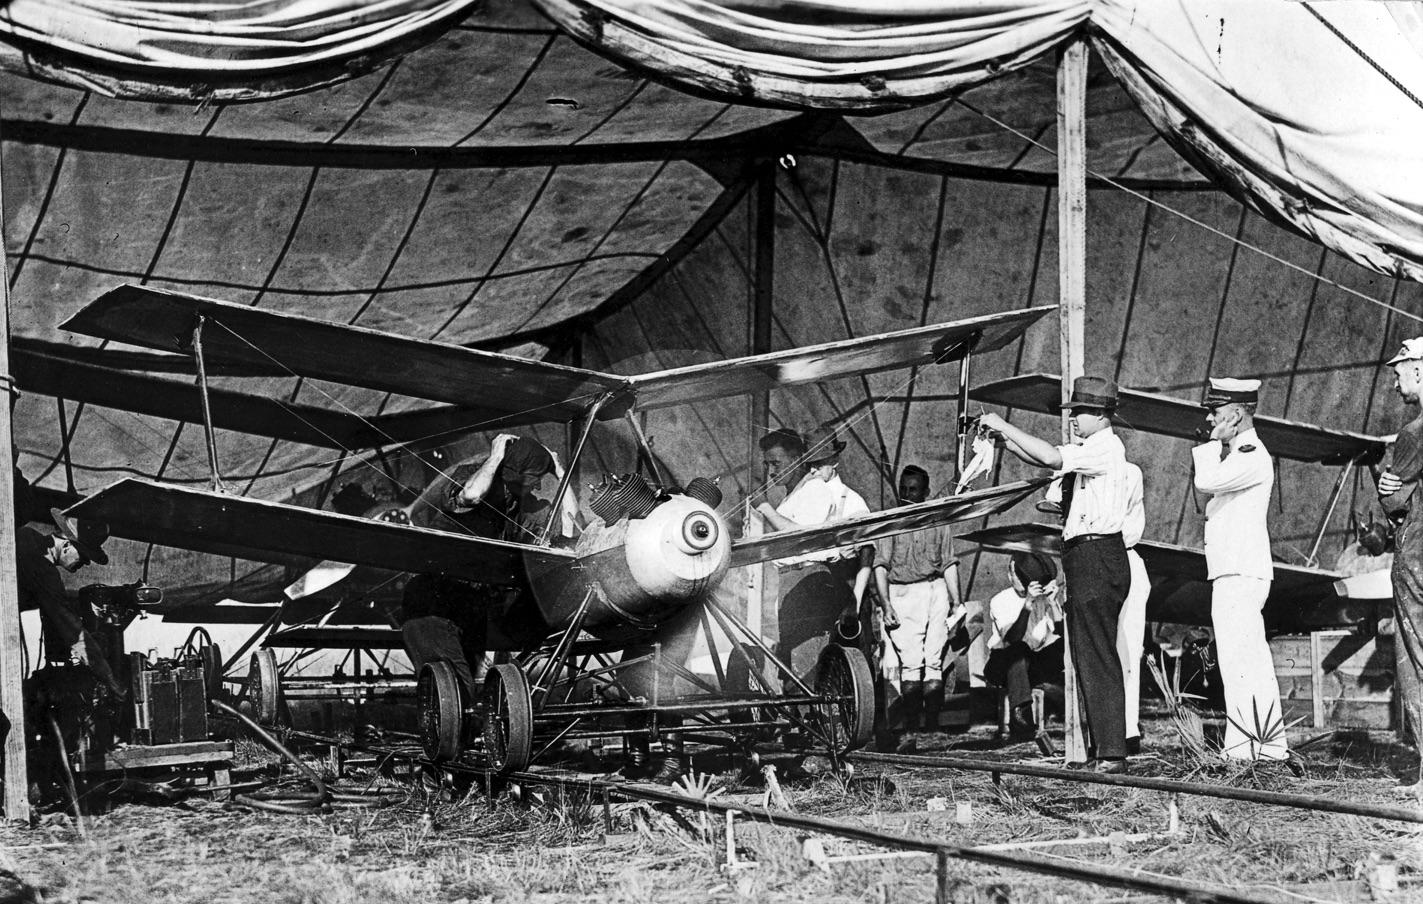
\includegraphics[width=0.3\textwidth,height=0.2\textwidth ]{figs/introducción/historia_drones/kettering-bug.jpg}
     \label{f:Kettering Bug}}
    \subfigure[Queen Bee]{
     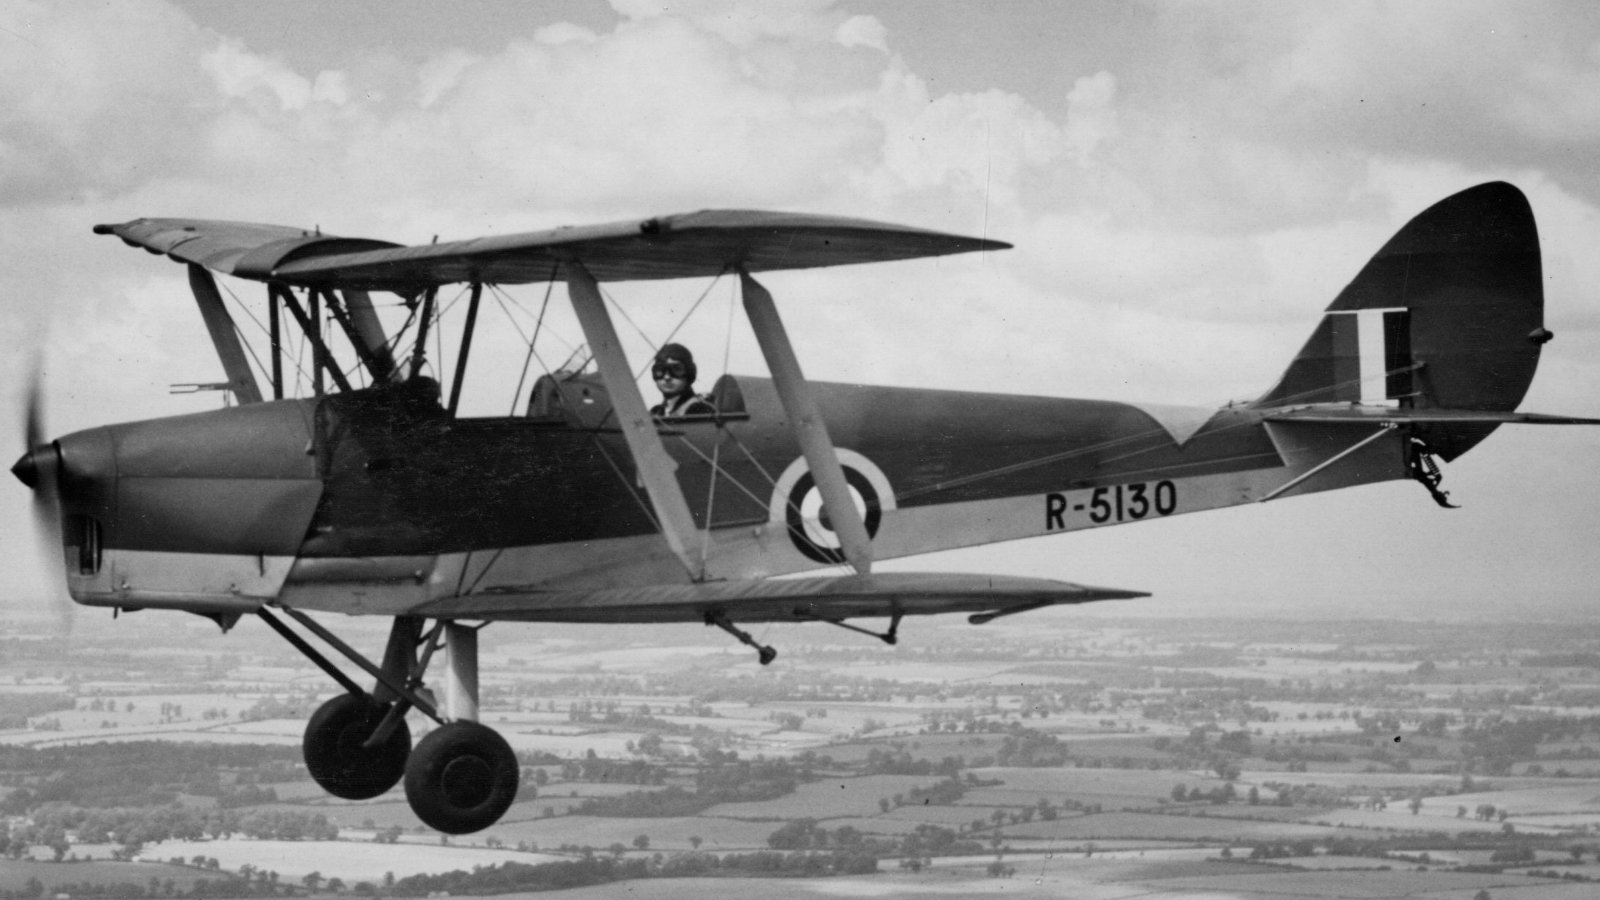
\includegraphics[width=0.3\textwidth,height=0.2\textwidth ]{figs/introducción/historia_drones/queen-bee.jpg}
     \label{f:Queen Bee}}
    \subfigure[V-1]{
      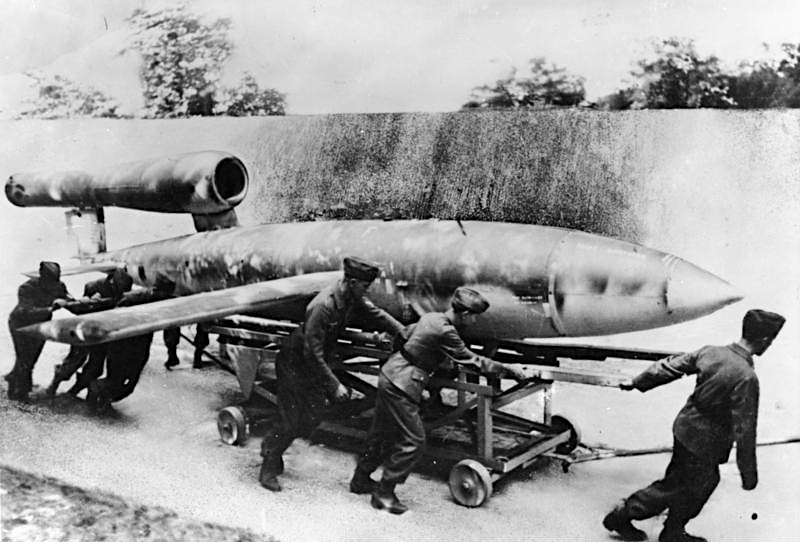
\includegraphics[width=0.3\textwidth,height=0.2\textwidth ]{figs/introducción/historia_drones/V-1.jpg}
      \label{f:V-1 "Flying Bomb"}}
    \subfigure[Proyect Aphrodite]{
      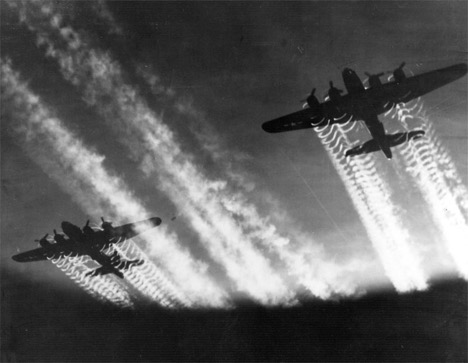
\includegraphics[width=0.3\textwidth,height=0.2\textwidth ]{figs/introducción/historia_drones/proyect-aphorite.jpg}
      \label{f:Proyect Aphrodite"}}
    \subfigure[Teledyne Ryan Firebee/Firefly]{
      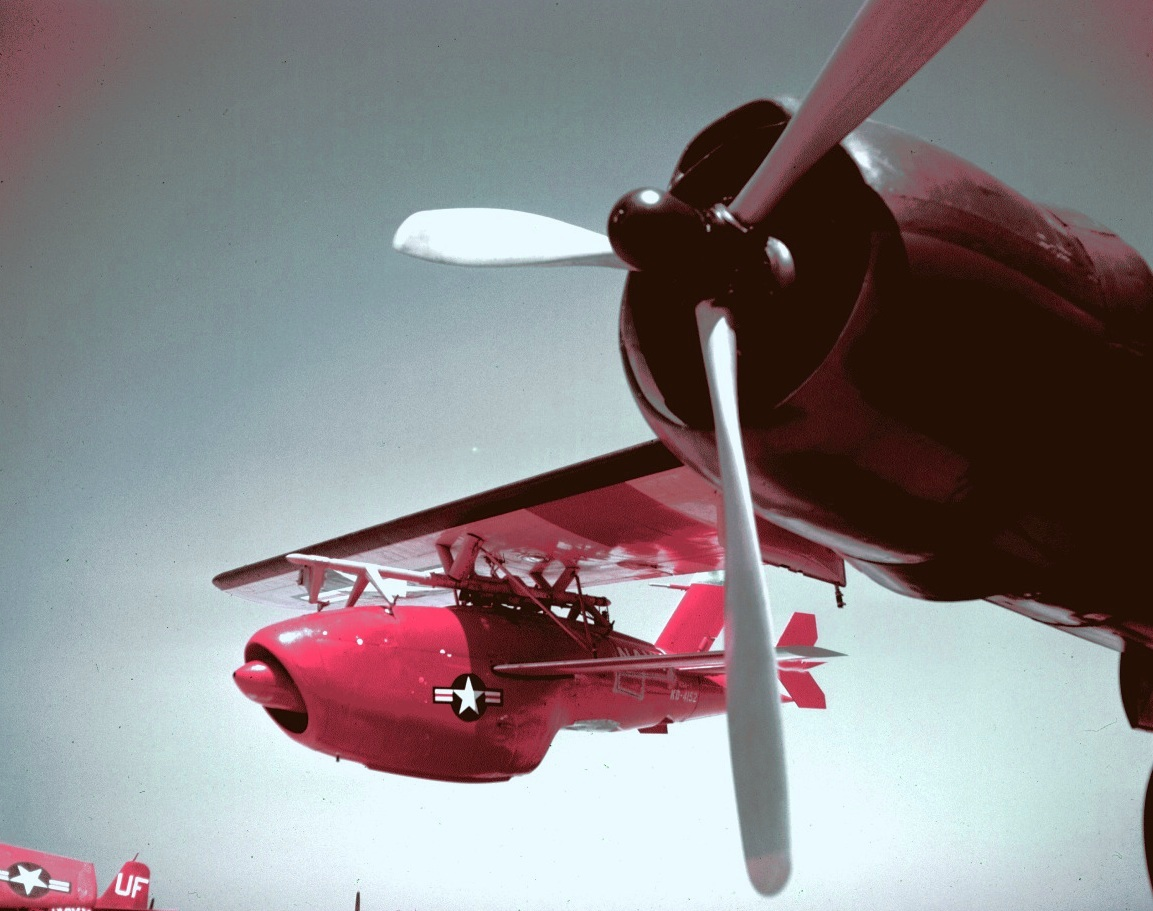
\includegraphics[width=0.3\textwidth,height=0.2\textwidth ]{figs/introducción/historia_drones/Firebee.jpg}
      \label{f:Teledyne Ryan Firebee/Firefly"}}
    \subfigure[Lockheed D-21]{
      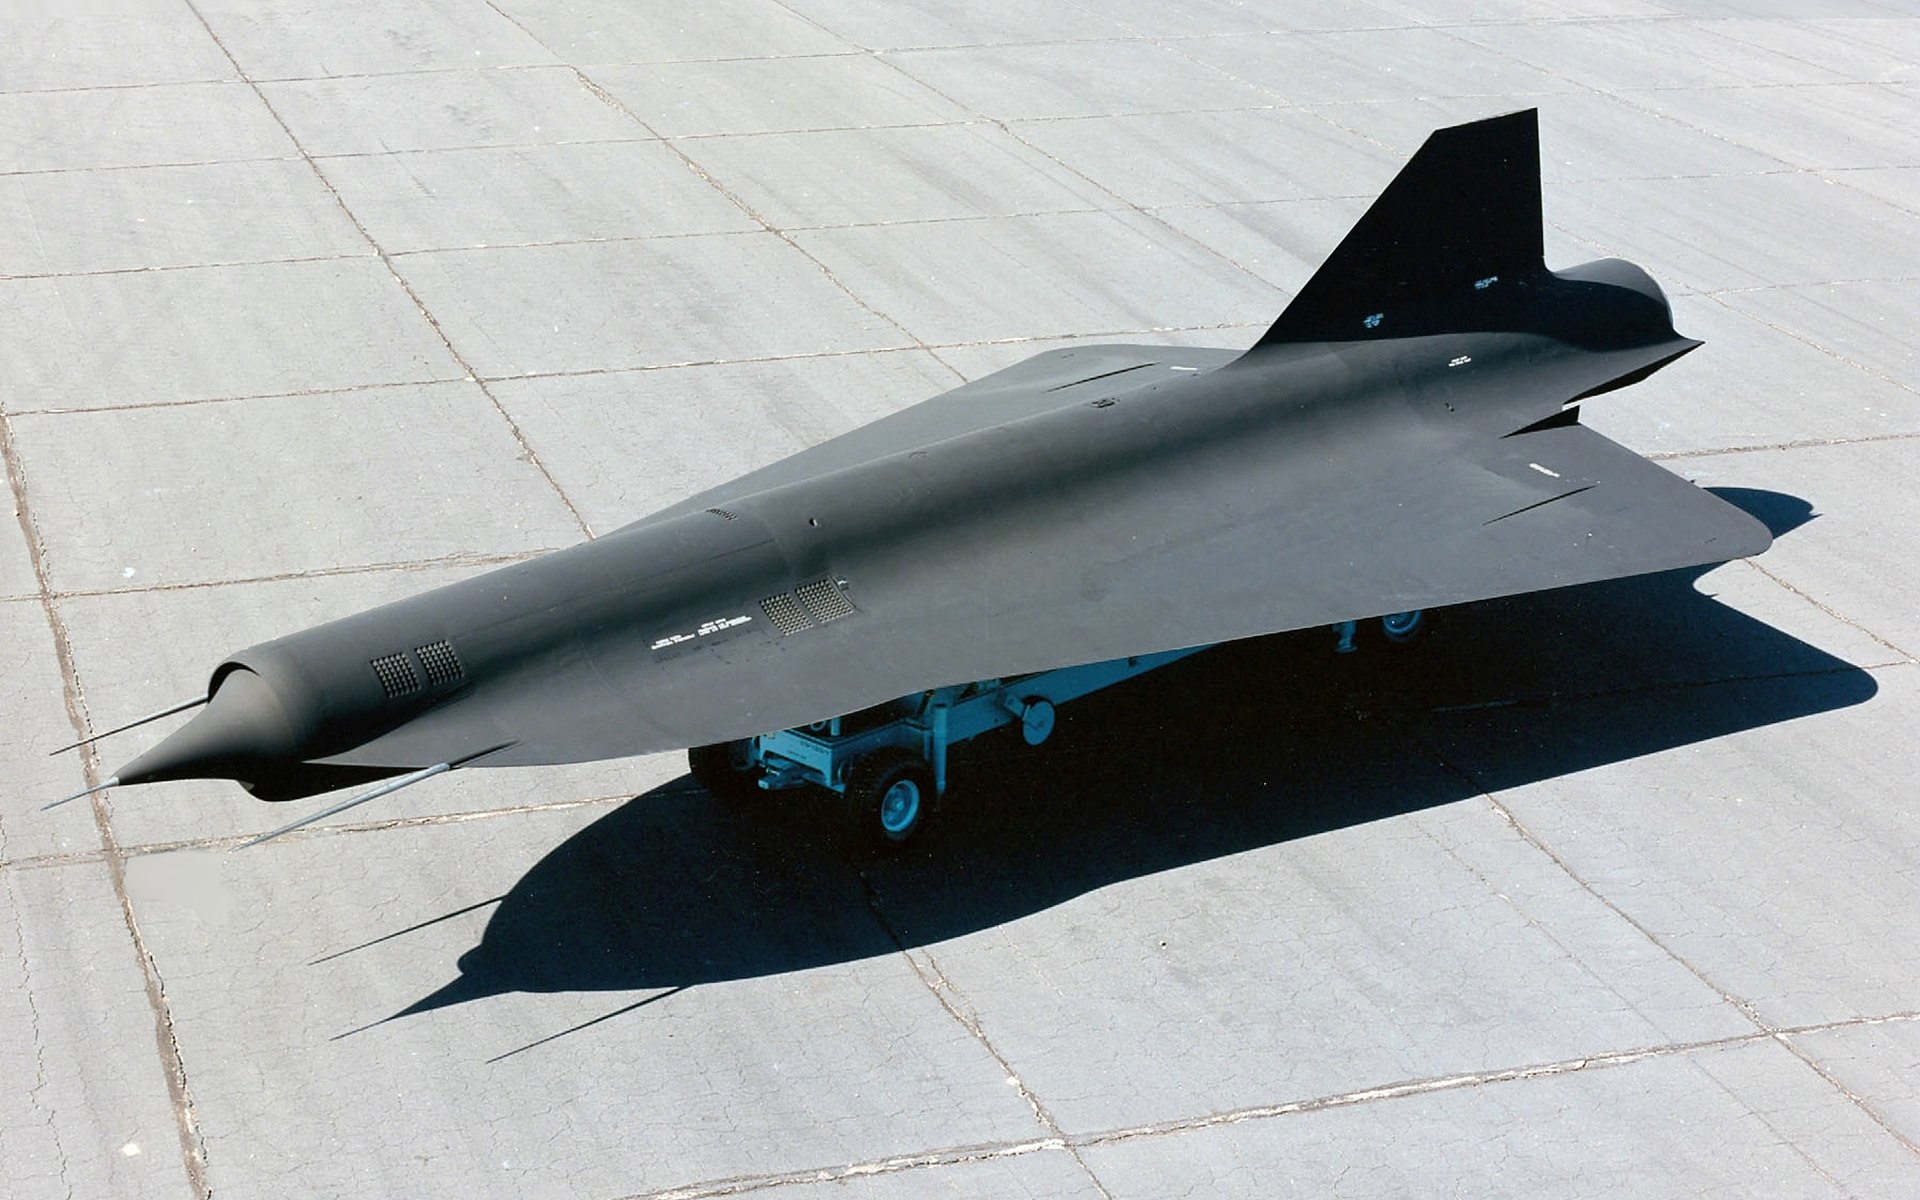
\includegraphics[width=0.3\textwidth,height=0.2\textwidth ]{figs/introducción/historia_drones/The_Lockheed_D-21.jpg}
      \label{f:Lockheed D-21"}}
    \subfigure[El Condor]{
      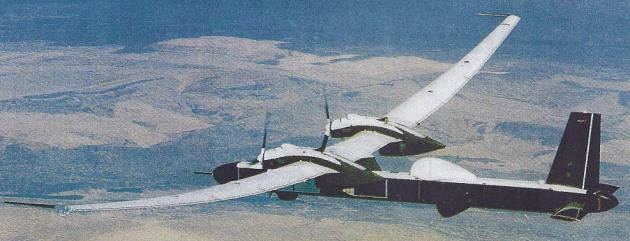
\includegraphics[width=0.3\textwidth,height=0.2\textwidth ]{figs/introducción/historia_drones/Boeing-Condor-UAV-23.png}
      \label{f:El Condor"}}
    \subfigure[Small UAV]{
      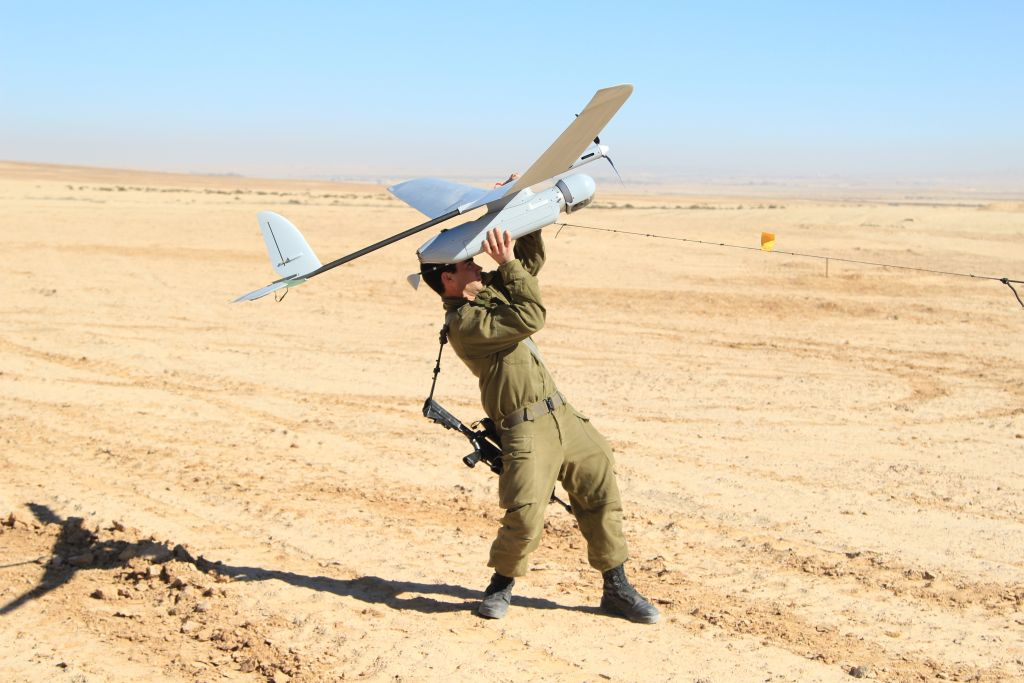
\includegraphics[width=0.3\textwidth,height=0.2\textwidth ]{figs/introducción/historia_drones/small-UAV.jpg}
      \label{f:small-UAV"}}
    \subfigure[Dron]{
      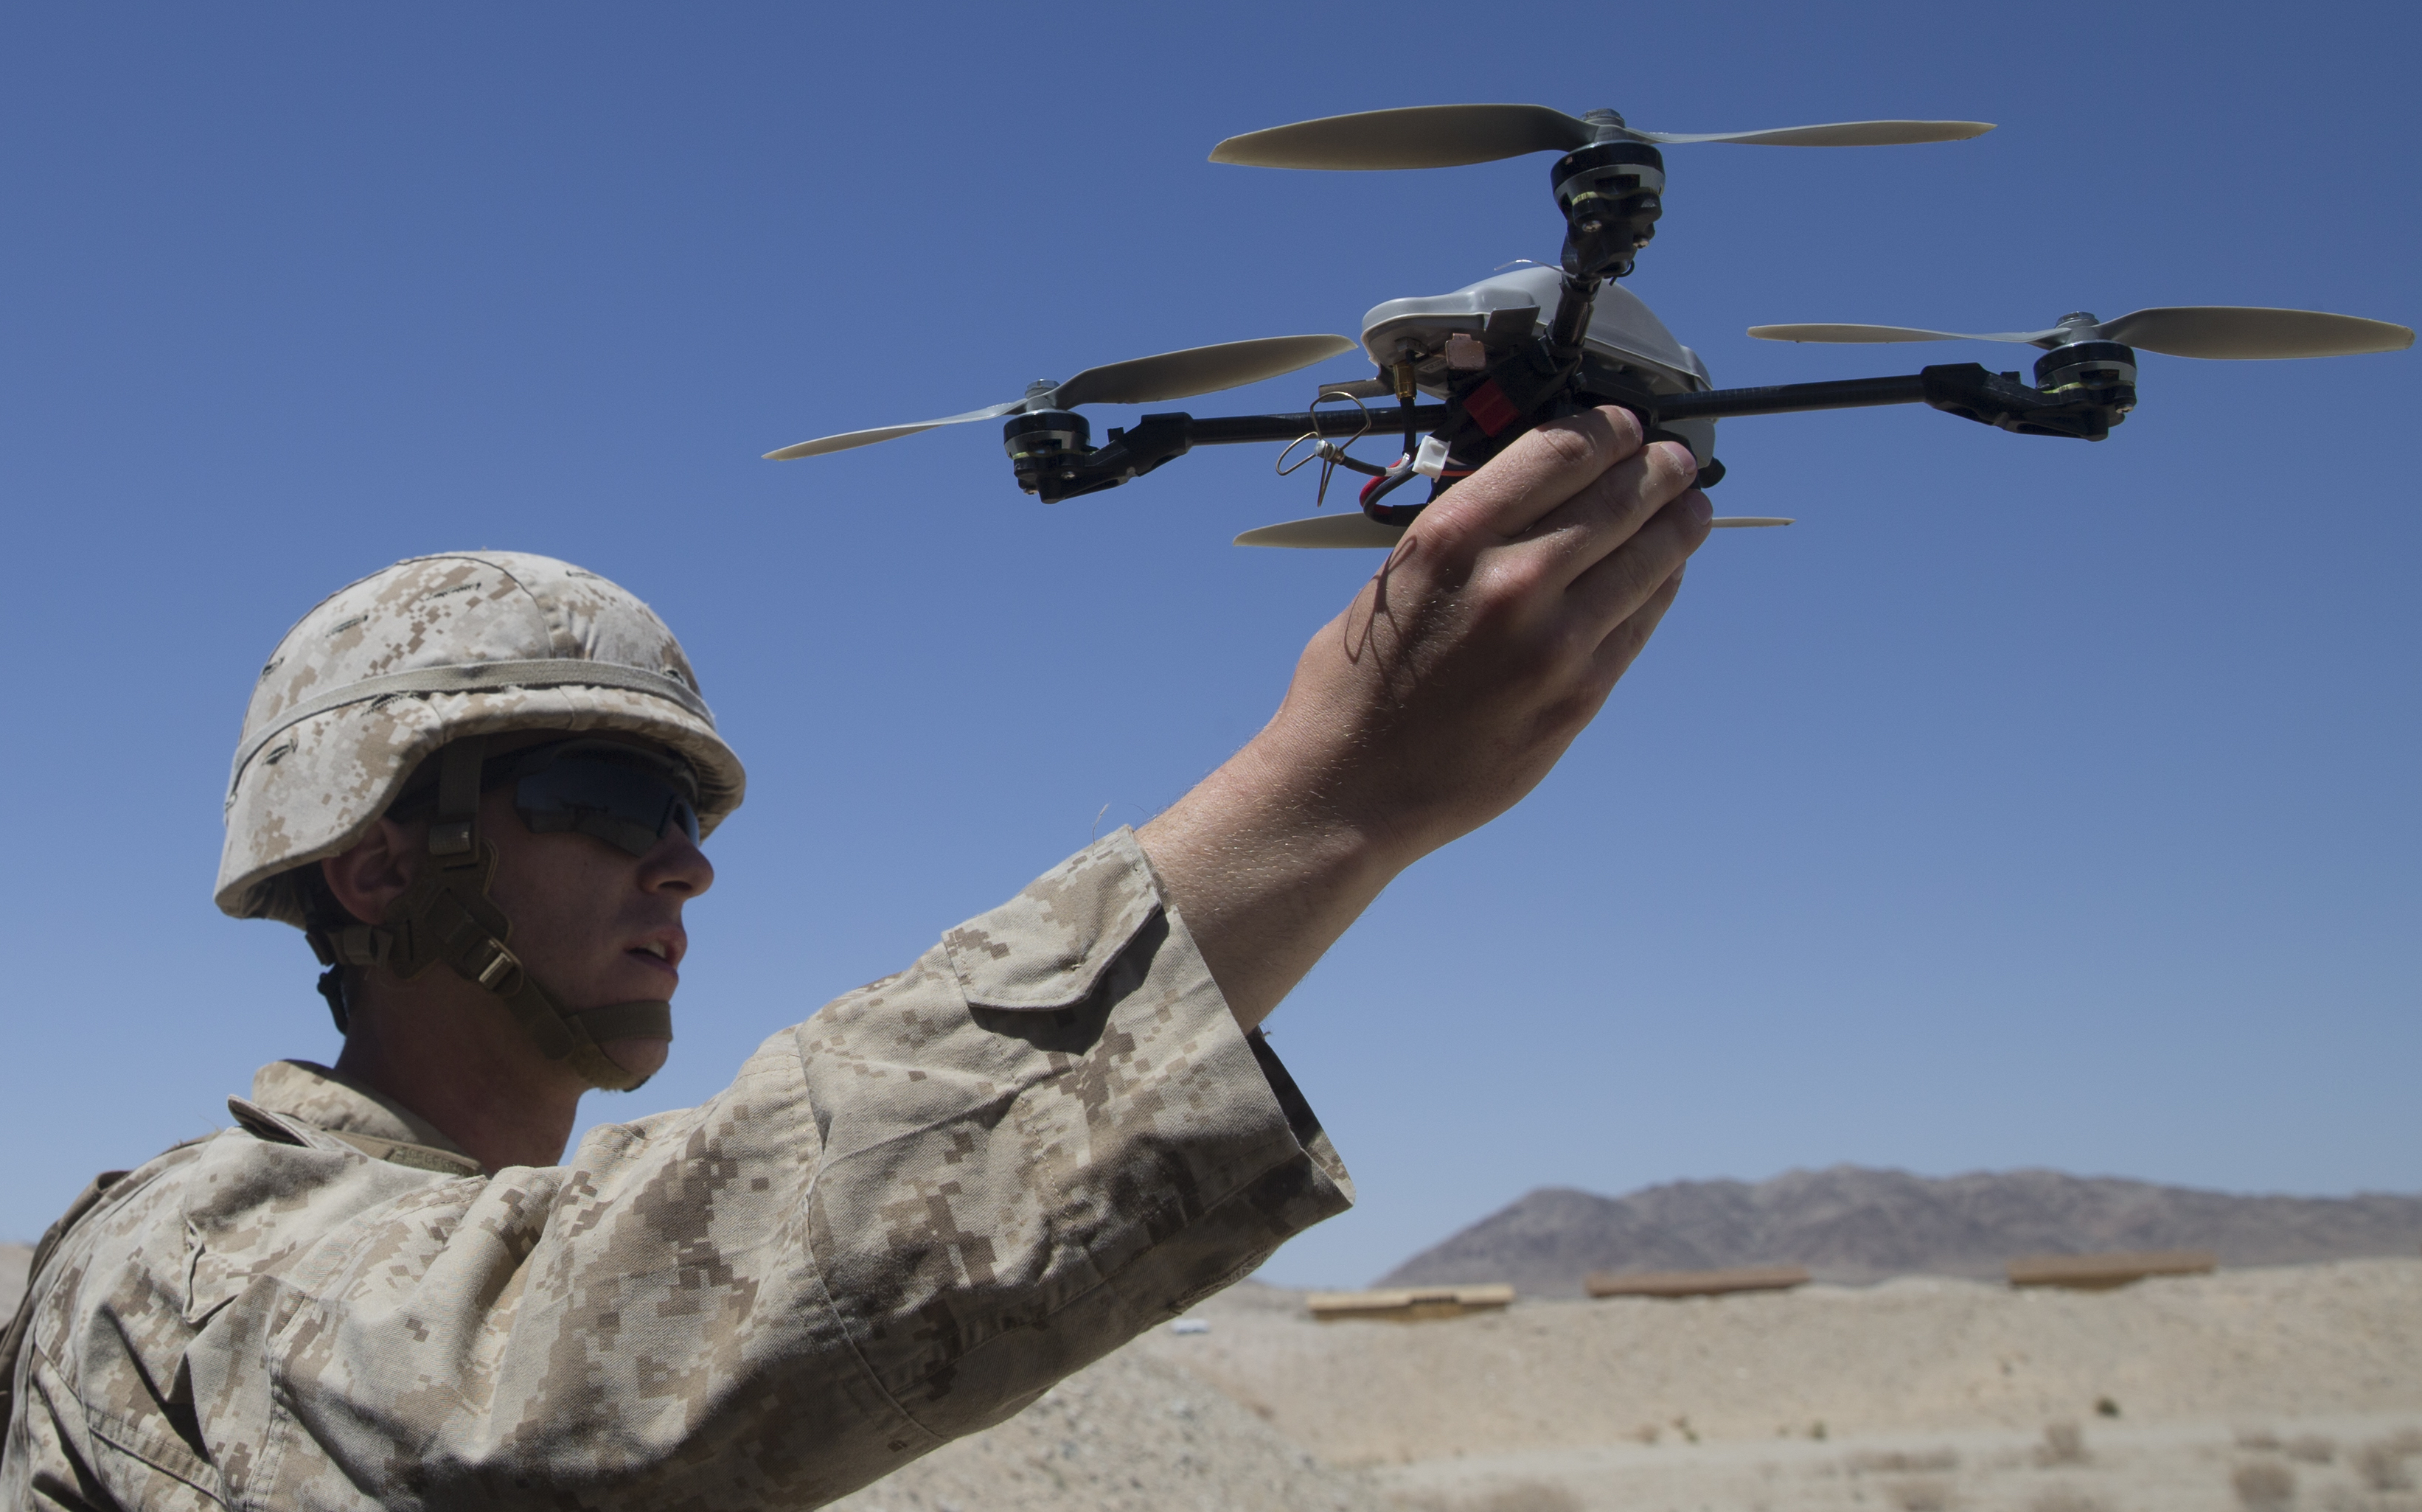
\includegraphics[width=0.3\textwidth,height=0.2\textwidth ]{figs/introducción/historia_drones/dron.jpg}
      \label{f:dron"}}
  \caption{Historia de los drones}
  \label{f:Drones}
  \end{center}
 \end{figure}

Cada vez es más común que los drones sean más sostificados y accesibles. Por ejemplo, el dron Ingenuity de la NASA se ha convertido en el primer vehículo aéreo autónomo en poder volar
sobre la superficie de otro planeta. Fue transportado a Marte mediante el rover Perseverance de la NASA, una vez fue posicionado el dron se elevó cerca de 3 metros realizando 
diferentes giros y desplazamientos tomando fotos a la superficie, teniendo la capacidad de escoger de forma autónoma los sitios de aterrizaje en el terreno marciano\footnote{\url{https://ciencia.nasa.gov/sistema-solar/finaliza-la-mision-del-helicoptero-ingenuity-en-marte/}}.
Este dron operaba de manera autónoma, controlado por sistemas de guía, navegación y control a bordo ejecutando los diferentes algoritmos desarrollados por la NASA. \newline

Uno de los grandes retos de este proyecto era demostrar la viabilidad del vuelo en la atmósfera de Marte, ya que su atmósfera esta compuesta por el 1\% de la densidad terrestre
dificultando el vuelo del dron. Sin embargo, gracias a su diseño ligero y a sus hélices especialmente diseñadas para crear suficiente sustentación en la atmósfera del planeta, el Ingenuity 
fue capaz de superar este desafío\footnote{\url{https://www.bbc.com/mundo/noticias-56738201}}. \newline
\begin{figure} [H]
  \begin{center}
    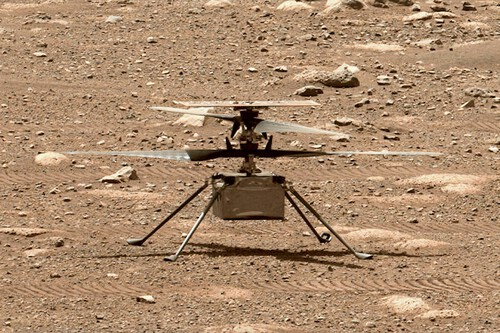
\includegraphics[scale=0.6]{figs/introducción/Ingenuity_II.jpeg}
  \end{center}
  \caption{El dron Ingenuity}
  \label{fig:Ingenuity}
\end{figure}\

Además, en su última fase, el Ingenuity realizó pruebas de vuelo experimentales para ampliar el conocimiento sobre cuáles eran sus límites aerodinámicos\footnote{\url{https://science.nasa.gov/mission/mars-2020-perseverance/ingenuity-mars-helicopter/}}.\newline

Otro ejemplo de uso de drones podemos tener el mantenimiento y control de redes eléctricas y otras infraestructuras. Algunas construcciones constan de grandes alturas y tamaños, lo que puede
dificultar el trabajo y su correcto mantenimiento. No obstante, estas tareas con los drones se agilizan y se vuelven más eficientes y robustas, porque permiten poder
inspeccionar dichas infraestructuras desde cerca sin poner en peligro a la seguridad de los operarios. 
Hay drones que se encargan en la monitorización de infraestructuras eléctricas. \newline

Unión Fenosa, la distribución eléctrica en España de Naturgy, en 2018 incorporó drones a sus instalaciones eléctricas para realizar labores de supervisión. Estos drones aportan 
soluciones optimizadas y eficientes en costes. Si tenemos en cuenta la longitud que puede tener las redes eléctricas, el uso de estos vehículos
autónomos facilita las tareas de supervisión equipados de cámaras de última generación permitiendo al operario observar en tiempo real el estado de las infraestructuras. Además de que los
drones podrían acceder a zonas de difícil acceso para comprobar daños y poder repararlos\footnote{\url{https://www.ufd.es/blog/primer-vuelo-de-un-dron-mas-alla-de-la-linea-visual/}}. \newline 


\begin{figure} [H]
  \begin{center}
    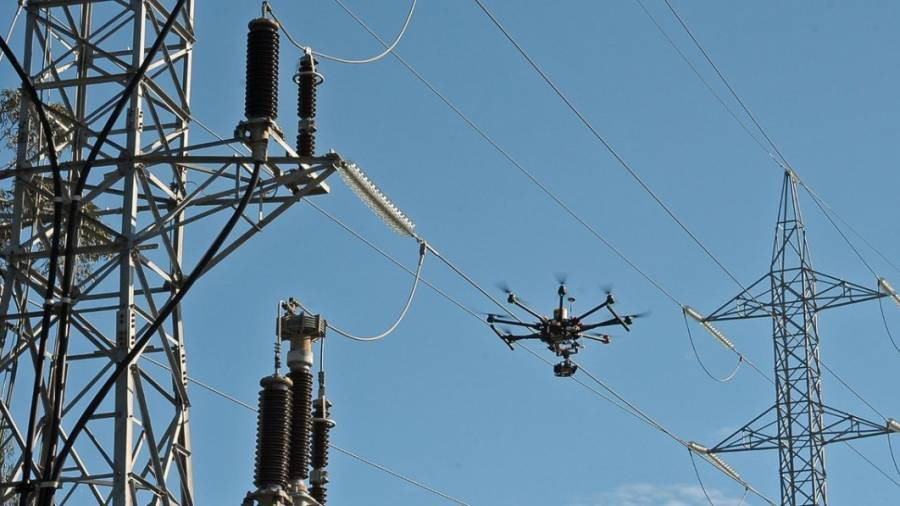
\includegraphics[scale=0.5]{figs/introducción/drones-red-electrica.jpg}
  \end{center}
  \caption{Drones en inspección eléctrica en Galicia}
  \label{fig:Fenosa}
\end{figure}\

Es importante mencionar que estos drones son teleoperados, lo que significa que requieren la intervención y el control directo de un operador humano para volar y realizar sus tareas 
de inspección y mantenimiento.\newline

Asimismo, Amazon ha estado trabajando en el desarrollo de drones autónomos para la entrega de paquetes durante varios años denominado así Prime Air\cite{AmazonPrimeAir}, 
que consiste en un sistema de entrega de paquetes utilizando estos vehículos. Durante este programa, han realizado diferentes pruebas de reparto de paquetes a clientes
en 60 minutos o menos. \newline

\begin{figure} [H]
  \begin{center}
    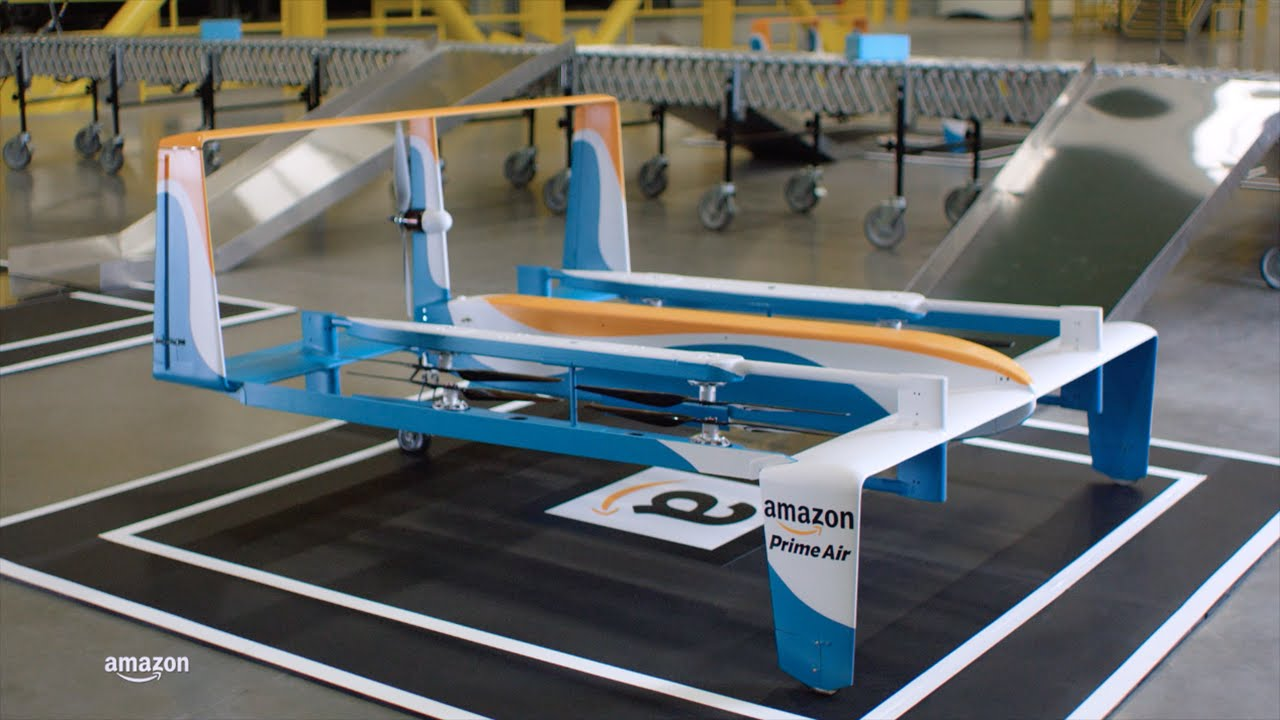
\includegraphics[scale=0.2]{figs/introducción/dron-amazon.jpg}
  \end{center}
  \caption{El primer prototipo de dron de Prime Air}
  \label{fig:PrimerPrimeAir}
\end{figure}\

A lo largo de los años, Amazon ha seguido investigando y diseñando nuevos modelos de drones como el dron autónomo MK27-2\footnote{\url{https://www.europapress.es/portaltic/gadgets/noticia-amazon-prime-air-comienza-entregar-pedidos-drones-estados-unidos-20221229115034.html}}. Fue el primer 
dron que utilizó Amazon para 
las primeras entregas dentro del programa Prime Air durante el año 2023, se basaba en un dron eléctrico capaz de entregar paquetes a los clientes en menos de una
hora y capaz de realizar vuelos evitando obstáculos como puede ser las chimeneas o las torres de telefonía aunque no puede realizar entregas durante tormentas, vientos fuertes, temperaturas
extremas o cualquier situación climatológica desfavorable. 

Este servicio solamente esta disponible para domicilios que tengan patios traseros que dispongan de espacio suficiente para que el dron pueda realizar el aterrizaje y la 
entrega del pedido.

\begin{figure} [H]
  \begin{center}
    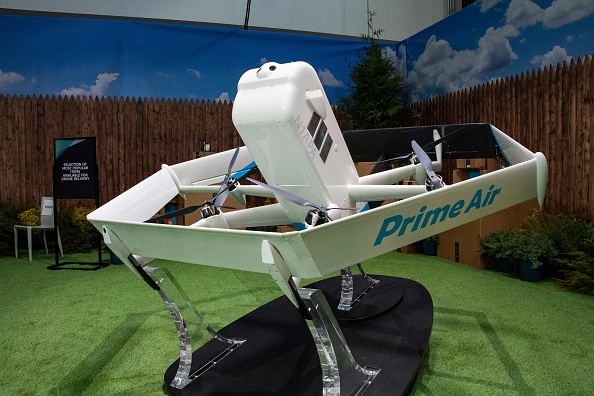
\includegraphics[scale=1.7]{figs/introducción/MK27-2.jpg}
  \end{center}
  \caption{El dron MK27-2}
  \label{fig:MK27-2}
\end{figure}\

Sin embargo, gracias al dron autónomo MK30 creado y diseñado por Amazon. Este pequeño dron será capaz de volar en diferentes condiciones climatológicas y 
constará de un sistema capaz de identificar y evitar obstáculos en el área de entrega. Una novedad de este dron en comparación con los anteriores modelos es que será capaz de aterrizar en espacios más reducidos lo que conlleva a que
este tipo de servicio pueda llegar a más vecindarios. \newline
Se tiene previsto que se llegue a probar en el año 2024 empezando por ciudades como Texas y California en Estados Unidos\footnote{\url{https://www.forbesargentina.com/innovacion/asi-nuevo-asombroso-dron-amazon-mk30-n42612}}. \newline

\begin{figure} [H]
  \begin{center}
    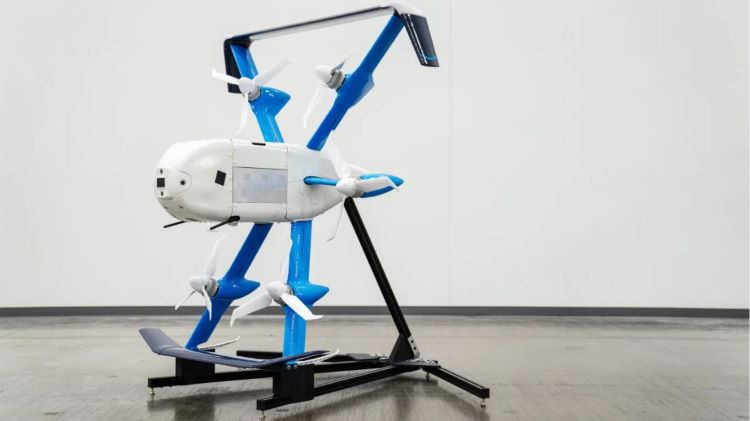
\includegraphics[scale=0.5]{figs/introducción/amazon-dron-mk30.jpg}
  \end{center}
  \caption{El dron MK30}
  \label{fig:MK30}
\end{figure}\

La navegación autónoma de drones sigue siendo un campo de investigación que busca permitir que los drones puedan volar de manera autónoma y segura.
Dentro de este ámbito, la detención y el seguimiento de carreteras se destacan como áreas prometedoras, un ejemplo de investigación sobre este campo, podemos 
tener este artículo \textit{Efficient Road Detection and Tracking for Unmmanned Aerial} \cite{article} que tiene como objetivo desarrollar un algoritmo de detección 
y seguimiento de carreteras específicas en videos capturados por vehículos aéreos no tripulados (UAV). Para la realizar la detección de carreteras utilizan 
un algoritmo denonimado Graph-Cut\footnote{\url{https://www.sciencedirect.com/topics/engineering/graph-cut-technique}}, 
que consiste en identificar y segmentar la imagen capturada por el dron para establecer la zona de interés,pero para obtener una segmentación más precisa y robusta de la carretera 
se combina con un modelo estadístico denonimado GMM\footnote{\url{https://builtin.com/articles/gaussian-mixture-model}} (Gaussian Mixture Model) para modelar las características de la imagen y representar regiones o clases
en la imagen (por ejemplo, carretera, fondo, vehículos).\newline

Una vez se realice la identificación de la carretera, se utilizará un algoritmo basado en homografía (tecnica geométrica), para ajustar la posición y la orientación del dron
en relación con la carretera. Este tipo de algoritmos de seguimiento de carreteras permite al dron seguir automáticamente las áreas que se definieron de la carretera. \newline

\begin{figure} [H]
  \begin{center}
    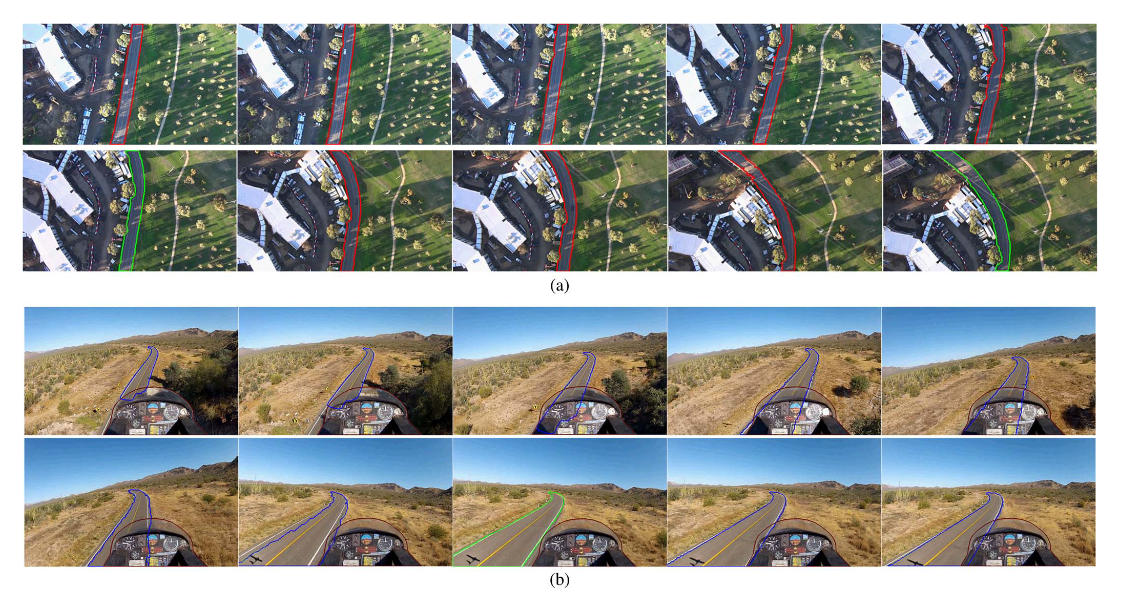
\includegraphics[scale=0.4]{figs/introducción/Efficient.png}
  \end{center}
  \caption{Resultados de detección y seguimiento de carreteras en Efficient Road Detection and Tracking for Unmmanned Aerial \cite{article}}
  \label{fig:Efficient}
\end{figure}\

Este enfoque puede tener aplicaciones como el monitoreo del tráfico y seguridad vial, seguimiento de vehículos terrestres o construcción de redes de carreteras para simulación. En un futuro cercano, puede que los drones sean más eficientes para las aplicaciones civiles y científicas incluyendo protección contra incendios forestales, misiones agrícolas, 
ayuda en catástrofes y más. 
Las demostraciones actuales del uso de los drones han revelado el potencial que pueden tener pero aun así el acceso al espacio aéreo sigue siendo un factor limitante. Con el paso del 
tiempo, se irá desarrollando nuevas tecnologías prácticas para poder permitir una integración segura en el espacio aéreo \cite{KrejciGarzon_2014}. \newline

En el artículo \textit{Automatic Damage Detection and Diagnosis for Hydraulic Structures Using Drones and Artificial Intelligence Techniques} \cite{rs15030615}, se explora el uso de drones
para monitorizar y diagnosticar daños estructurales en presas hidráulicas. El objetivo principal de este estudio es detectar y evaluar el estado de  grietas en estas estructuras. Para lograrlo, 
se emplean algoritmos de visión por computadora e inteligencia artificial. 
En particular, se utiliza una red neuronal llamada Xception \cite{Deeplabv3} junto con algoritmos de segmentación semántica de imágenes para detectar áreas afectadas. Los resultados experimentales, 
presentados en la figura \ref{fig:Hidraulica}, demuestran la eficacia de esta detección de daños en las presas hidráulicas mediante el uso de técnicas de visión e inteligencia artificial. 

\begin{figure} [H]
  \begin{center}
    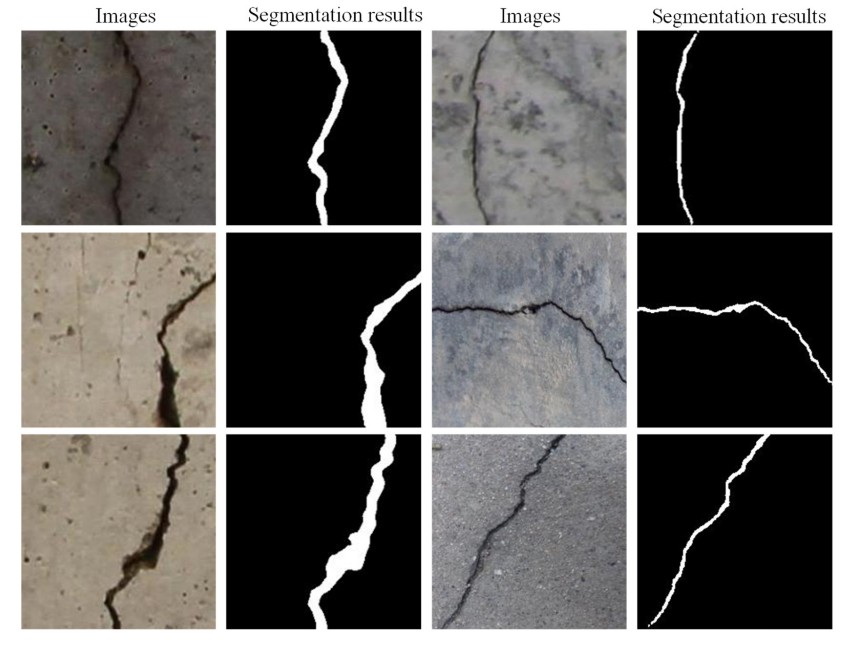
\includegraphics[scale=0.4]{figs/introducción/grietas.png}
  \end{center}
  \caption{ Demostración de la identificación de diferentes tipos de grietas \cite{Deeplabv3}}
  \label{fig:Hidraulica}
\end{figure}\

En resumen, los drones son una tecnología emergente con un potencial significativo
para transformar una variedad de industrias. Sin embargo, también plantean desafíos únicos que deben ser abordados a medida que se integran más plenamente en nuestra
sociedad. Con el desarrollo continuo de la tecnología de los drones y la evolución de las
regulaciones, es probable que veamos un aumento en la variedad de las aplicaciones de
los drones en el futuro. 


\section{La inteligencia artificial en la navegación autónoma de drones}
\label{sec:IA}

La incorporación de inteligencia artificial en el mundo de la robótica y en especial en los drones desempeña un papel crucial en la navegación autónoma, permitiéndoles tomar decisiones en tiempo real y adaptarse 
a entornos cambiantes de manera eficiente. Permitiendo a los drones poder aprender de sus experiencias y entender e interactuar con el entorno en el que se encuentran de una manera más
óptima. \newline

Los drones equipados con IA de percepción o de control pueden realizar vuelos de precisión, mantener la estabilidad incluso en condiciones adversas como fuertes vientos, y evitar obstáculos 
de forma dinámica. Esto es posible gracias a la combinación de datos sensoriales junto con los algoritmos de IA, lo que permite 
al dron interpretar su entorno y tomar decisiodecisiones en tiempo real. Uno de los enfoques más destacados en la navegación autónoma de drones es el aprendizaje automático. Este enfoque permite a los drones mejorar su objetivo a través de la experiencia 
y los datos recopilados durante el vuelo. 

\begin{figure} [H]
  \begin{center}
    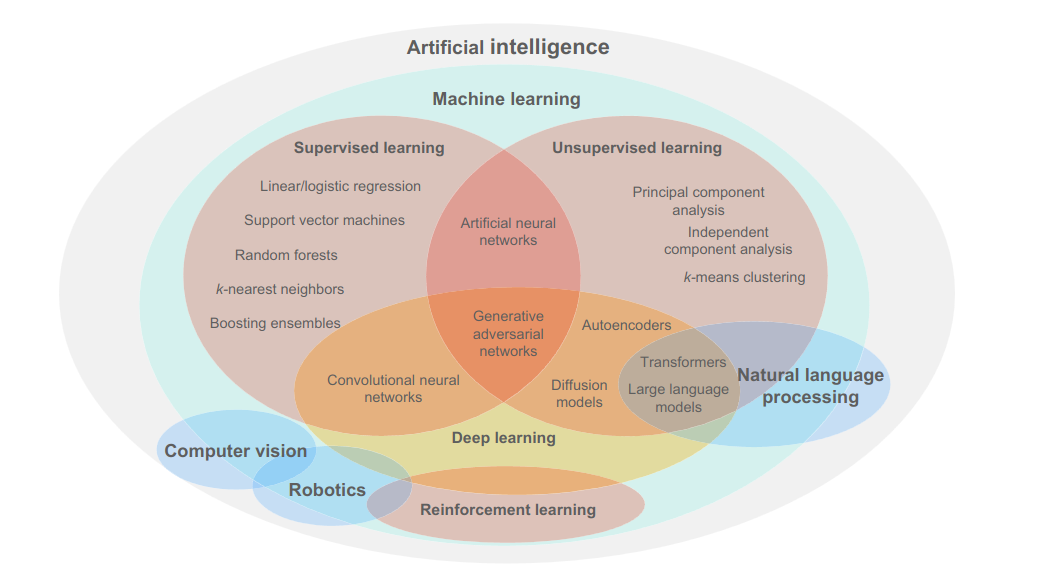
\includegraphics[scale=0.4]{figs/introducción/IA-diagrama.png}
  \end{center}
  \caption{Clasificación de Inteligencia Artificial \cite{IA}}
  \label{fig:ClasificaciónIA}
\end{figure}
\newpage

Por ejemplo, las CNN son capaces de analizar imágenes capturadas por las cámaras a bordo del dron para identificar obstáculos, 
peatones o vehículos. Un tipo de aplicación de uso de redes neuronales es la detección y clasificación de malas hierbas como se muestra 
en el artículo \textit{Weed detection and classification using UAVs and deep neural networks: mapping for localized treatment} \cite{CSIC}. Mediante el sensor de la cámara, el dron es capaz de capturar imágenes en tiempo real 
para más adelante usar la red neuronal CNN YOLOv8 \cite{Ultralytics_YOLOv8} para detectar y clasificar las diferentes hierbas que puede haber en un campo de cultivo. Este tipo de aplicación es bastante útil para la inspección
agrícola ya que los drones pueden crear mapas detallados que permiten a los agricultores aplicar herbicidas de manera más eficiente y precisa, también este tipo de aplicación puede
ser útil para tener una monitorización general sobre la salud del cultivo. El resultado se puede visualizar en la figura \ref{fig:malas hierbas}.\newline 

\begin{figure} [H]
  \begin{center}
    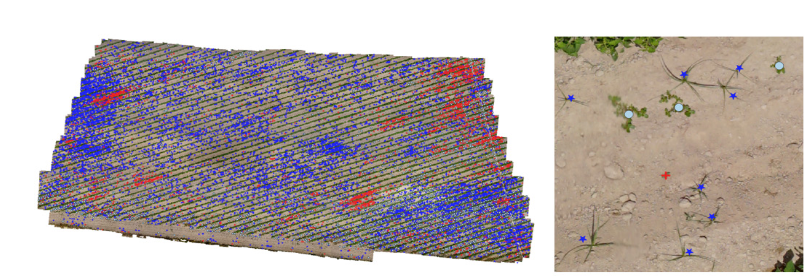
\includegraphics[scale=0.55]{figs/introducción/malashierbas.png}
  \end{center}
  \caption{Resultados de la detección y clasificación de malas hierbas en un cultivo \cite{CSIC}}
  \label{fig:malas hierbas}
\end{figure}

Por otro lado, reinforcement learning (RL) \cite{6025669} es una técnica dentro del aprendizaje automático que es interesante utilizar en la navegación autónoma de drones. Esta metodología permite
a los drones aprender a planificar rutas de forma autónoma, mejorando su desempeño a mediante un esquema de penalizaciones y recompensas permitiendo
así al dron poder tomar decisiones decisivas en situaciones puntuales. En el artículo \textit{Vision based drone obstacle avoidance by deep
reinforcement learning} \cite{ai2030023} precisamente se utiliza un algoritmo de RL para la evitación de obstáculos en un espacio continuo y se llega a conseguir que con estos
tipos de algoritmos que un dron pueda llegar aprender comportamientos y tomar decisiones por él mismo. 

\begin{figure} [H]
  \begin{center}
    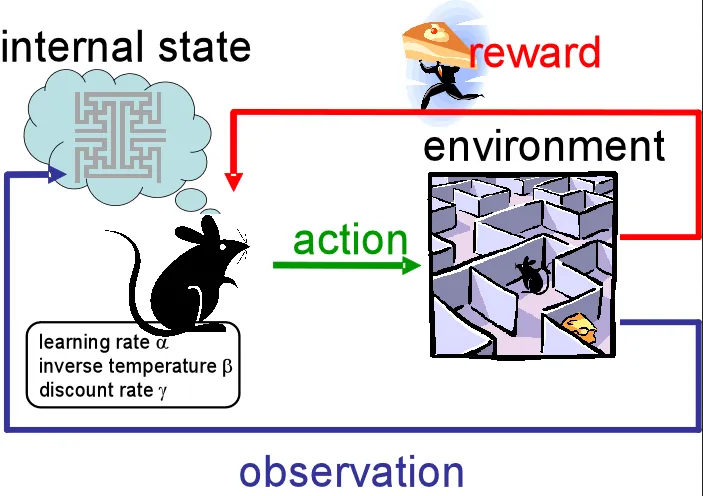
\includegraphics[scale=0.4]{figs/introducción/RL.png}
  \end{center}
  \caption{Esquema de Reinforcement Learning \cite{BecomingHuman_RL_Basics}}
  \label{fig:Reinforcement Learning}
\end{figure}\



En conclusión, la inteligencia artificial puede ser fundamental en la navegación autónoma de drones al permitirles percibir su entorno, podemos tomar decisiones y planificar acciones 
de manera anticipada y autónoma. A medida que vayamos avanzando, se espera que los drones tengan más sistemas de inteligencia artificial abordo para cubrir una amplia gama de tareas
de manera autónoma, lo que abriría nuevas fronteras en campos como el rescate, la vigilancia, la logística y la exploración, y que promete seguir transformando la forma en que 
interactuamos con el espacio aéreo en un futuro. 

\newpage
\section{Navegación autónoma en Airsim basada en inteligencia artificial y aprendizaje por refuerzo}
\label{sec:Navegación autónoma}

En este trabajo realizaremos un algoritmo basado en navegación autónoma para drones por entornos de carreteras sin intervención humana. Nuestro enfoque se basa en 
combinar la inteligencia artificial (IA) y aprendizaje por refuerzo (RL) para lograr vuelos autónomos y seguros, además de utilizar técnicas de procesamiento de imágenes 
y visión para detectar y segmentar las carreteras en las imágenes capturas por el dron permitiendo establecer regiones de interés específicas para la navegación 
autónoma.\newline

Este tipo de comportamientos pueden tener aplicaciones potenciales como monitorizar carreteras en la seguridad vial identificando los diferentes carriles de las carreteras y sus vehículos
en tiempo real, entrega de paquetes de manera autónoma siguiendo rutas de carreteras o vigilancia de accidentes en áreas de carreteras. \newline

En conclusión, con este trabajo de investigación buscamos impulsar el uso de la tecnología de drones en la seguiridad, planificación y eficiencia en el ámbito de las carreteras. 



%\chapter{Objetivos}
\label{cap:capitulo2}

En esta sección se describirá el problema a resolver junto con los objetivos y requisitos pautados en el desarrollo del TFG

\section{Descripción del problema}
\label{sec:descripcion}

El objetivo principal de este TFG, es desarrollar un comportamiento de navegación autónoma basado en 
aprendizaje por refuerzo e inteligencia artificial, en el que el dron sea capaz de navegar de una manera robusta por escenarios urbanos. El enfoque de este trabajo de investigación 
se centra en la creación de una solución eficiente y completa ante la problemática que puede llegar a tener la navegación autónoma, se 
muestra un comportamiento capaz de realizar el seguimiento de un carril para demostrar la complejidad de mantener una trayectoria estable 
y precisa utilizando un dron. 

A continuación, se definen los siguientes subobjetivos: 

\begin{enumerate}
    \item Estudio del arte de los drones con el objetivo de definir las posibilidades que puede ofrecer y definir 
    la navegación autónoma dentro del entorno en el que se desarrollará el TFG. 
    \item Análisis y uso de un sistema perceptivo basado en redes neuronales en la navegación autónoma de drones.
    \item Desarrollo  de un sistema de control para drones utilizando técnicas de aprendizaje por refuerzo para lograr una navegación 
    autónoma y eficaz.
    \item Análisis y desarrollo de una aplicación de navegación autónoma de drones basándonos en el seguimiento de un carril.
    \item Análisis y comparativas de los diferentes comportamientos desarrollados en este trabajo con el fin de 
    lograr resultados interesantes acerca de la utilización de redes neuronales y aprendizaje por refuerzo en la navegación autónoma de drones.
\end{enumerate}
\newpage
\section{Requisitos}
\label{sec:requisitos}

Los requisitos que han de cumplirse en este trabajo son: 
\begin{enumerate}
    \item Uso del vehículo UAV en el entorno de simulación fotorrealista Airsim junto a UnRealEngine.
    \item Utilización del middleware robótico ROS para así garantizar la interoperabilidad del trabajo en otro tipo de escenarios permitiendo
    la reutilización del proyecto en diversas aplicaciones. 
    \item Comportamiento robusto y en tiempo real para garantizar la navegación del dron dentro del circuito urbano.
    \item Los sistemas desarrollados deben ser reactivos para poder reaccionar a su entorno de manera concisa y eficiente durante
    la navegación en tiempo real.
    \item Uso del algoritmo de Q-learning para la navegación autónoma del dron. 
\end{enumerate}


\section{Metodología}
\label{sec:metodologia}

Este trabajo, comenzó oficialmente en Septiembre del 2023 aunque en Diciembre del 2022 se plantearon varias ideas a desarrollar, y se finalizó en Mayo del 2024.

La metodología que se llevo a cabo fue:

\begin{enumerate}
    \item Reuniones semanales mediante Teams\footnote{\url{https://www.microsoft.com/es-es/microsoft-teams/group-chat-software}} con una duración de media o una hora, con el fin de tener un control semanal y pactar los objetivos semanales a seguir. Gracias a estas reuniones, se tenia una organización global del proyecto. 
    \item Contacto vía email de la universidad con el fin de solventar problemas urgentes. 
    \item Utilización de la metodología Kanban\footnote{\url{https://canalinnova.com/que-es-y-para-que-sirve-el-kanban-definicion-fases-y-pasos/}}: Este tipo de metodología consiste en crear un flujo de trabajo
    en equipos mediante la gestión visual. Se compone de varias fases:
  
    \begin{itemize}
      \item \textbf{Fase 1: Inicio del proyecto}. Consiste en marcar los objetivos que se deben seguir dentro del proyecto junto la asignación e identificación de tareas. En esta fase, 
      definimos el tipo de aplicación que se iba a seguir que es la navegación autónoma de drones considerando un entorno de simulación de carreteras, la infraestructura, los tipos 
      de algoritmos a seguir y las analíticas de los comportamientos desarrollados durante el TFG. 
      \item \textbf{Fase 2: Diseño del tablero Kanban}. Se crea un tablero en donde se visualizarán las tareas y su estado. Cada tarea se definen en las columnas del tableros las
      tareas que se deben realizar junto con indicadores visuales como se muestra en la figura 
      \item \textbf{Fase 3: Implementación del tablero Kanban}. Se asignan las tareas a realizar y se establecen límites de trabajo en progreso como el tiempo de desarrollo para 
      completar dicha tarea. 
      \item \textbf{Fase 4: Seguimiento y mejora continua}. Se realiza un flujo continuo y constante del trabajo identificando nuevas soluciones para mejorar la eficacia y la 
      productividad hasta de poder cambiar estrategias existentes por nuevas alternativas previamente definidas. En este trabajo hemos realizo varias tareas y seguimientos para encontrar
      la mejor solución ante el problema a resolver.

      
      A lo largo del desarrollo de este TFG, se marcaron estas 4 fases permitiendo cambios y mejoras continuas hasta llegar al resultado final.

    \end{itemize}
  
    \begin{figure} [H]
        \begin{center}
          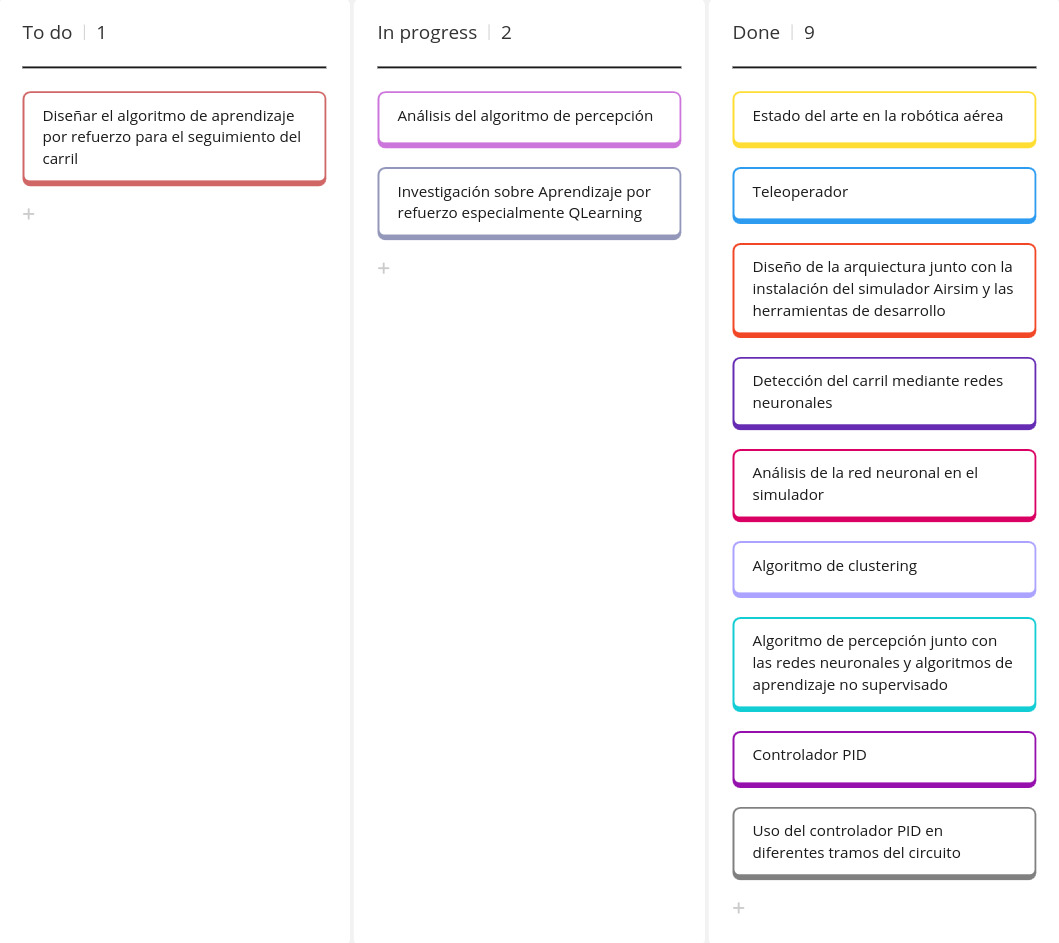
\includegraphics[scale=0.3]{figs/objetivos/Kanban3.jpg}
        \end{center}
        \caption{Ilustración del tablero Kanban durante el desarrollo del TFG}
        \label{fig:Espiral}
        \vspace{-1.5em}
      \end{figure}
  
    \item Tener un control de versiones mediante la plataforma GitHub\footnote{\url{https://github.com/RoboticsLabURJC/2022-tfg-barbara-villalba}}, con el objetivo de tener un almacenamiento de código y respaldos de ello.  
    \item El uso de un blog \footnote{\url{https://roboticslaburjc.github.io/2022-tfg-barbara-villalba/}}, en el cual se describió brevemente los pasos que se siguieron para el desarrollo del TFG.
\end{enumerate}

\begin{figure} [H]
    \begin{center}
      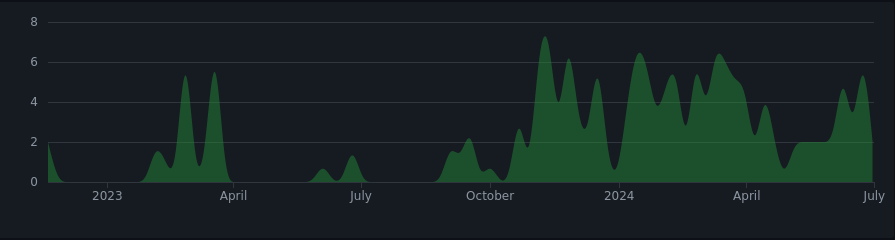
\includegraphics[width=0.7\textwidth,height=0.3\textwidth]{figs/objetivos/github.png}
    \end{center}
    \caption{Seguimiento de trabajo en GitHub}
    \label{fig:github}
    \vspace{-1.5em}
  \end{figure}


\section{Plan de trabajo}
\label{sec:plantrabajo}

Finalmente, los pasos a seguir de este trabajo han sido: 
\begin{enumerate}
    \item Comienzo del trabajo. 
    \begin{itemize}
        \item Búsqueda del problema a desarrollar y análisis del estado del arte del uso de los drones en aplicaciones robóticas.
        \item Instalación de las diferentes librerías y aplicaciones de software. 
        \item Preparación de configuración de toda la infraestructura, teniendo un análisis y estudio de comunicaciones para poder comenzar con el desarrollo. 
    \end{itemize}
    \item Desarrollo: Una vez se tuvo listo toda la infraestructura tanto de comunicaciones como de librerías de software, se dio a pie el comienzo del desarrollo del código
        \begin{itemize}
            \item En primer lugar, se desarrollo un teleoperador sencillo del drone para ver el funcionamiento del vehículo y dicho comportamiento.
            \item Una vez finalizada la tarea del teleoperador, se comenzó con los algoritmos de percepción de detención de carril mediante redes neuronales.
            \item Análisis y comparación de los resultados de los diferentes modelos que ofrece la red neuronal escogida con el propósito de tener la mejor solución. 
            \item El siguiente paso fue estudiar la posibilidad de tener un algoritmo de aprendizaje no supervisado llamado clustering para clasificar las diferentes lineas que aparezcan en el escenario de la carretera.
            \item Desarrollo del algoritmo de percepción junto con los dos puntos anteriormente mencionados.
            \item Con el fin del algoritmo de percepción, se comenzó el desarrollo de un controlador sencillo PID para ver el funcionamiento de la percepción y de la navegación en el vehículo. 
            \item A continuación, fue la programación del algoritmo de aprendizaje por refuerzo para el seguimiento del carril.
        \end{itemize}
    \item Evaluación: Se realizo la comparativa de los resultados obtenidos en el aprendizaje por refuerzo.
        
    \item Redacción de la memoria del trabajo para la documentación de todo el proceso de investigación realizado. 
\end{enumerate}



%\chapter{Plataforma de desarrollo}
\label{cap:capitulo3}

En este capítulo hablaremos sobre qué tecnologías hemos utilizado durante el desarrollo de este trabajo junto con el lenguaje de programación y las librerías utilizadas.
\section{Lenguaje de programación}
\label{sec:programación}
\subsection{Python}
\label{sec:python}
Para el desarrollo de este TFG, hemos utilizado como lenguaje de programación Python. Python\footnote{\url{https://www.python.org/}} es un lenguaje de programación interpretado, 
de tipado dinámico y orientado a objetos,
utilizado para el desarrollo de software, aplicaciones web, data science y machine learning (ML).  
Fue creado por Guido van Rossum\footnote{\url{https://gvnrossum.github.io/}} en 1989, el nombre de "Python" se inspiró en el programa de televisión británico 
"Monty Python's Flying Circus". \newline

Este lenguaje con los tiempos se ha convertido en uno de los lenguajes más populares del mundo, esto se puede deber a su sintaxis sencilla, clara y legible, aparte 
de estos beneficios también presenta una amplia gama de bibliotecas y marcos de trabajo. Además,se trata de un lenguaje de programación 'open source' (código abierto) y está disponible bajo
una licencia de código abierto aprobada por la Iniciativa de Código Abierto (OSI), esto significa que Python es libre de usar, distribuir y modificar, incluso para uso
comercial. \newline

También a de destacar, la facilidad que puede ser la instalación de dicho lenguaje en sistemas operativos como Linux o Windows. \newline

En el caso de este TFG, se utiliza Python3 para todo el desarrollo del código junto con el middleware robotico ROS (veáse la sección \ref{sec:ros}) y para el desarrollo
de los diferentes algoritmos. 
\newline

\begin{code}[h]
\begin{lstlisting}[language=Python]
  def factorial(n):
    if n == 0:
        return 1
    else:
        return n * factorial(n-1)

print(factorial(5))  # Output: 120

\end{lstlisting}
\caption[Ejemplo de código en Python de una función para calcular el factorial de un número]{Ejemplo de código en Python de una función para calcular el factorial de un número}
\label{cod:codejemplo}
\end{code}  


Para el desarrollo del sistema de percepción, hemos utilizado varías librerías mediante el lenguaje de programación Python para poder
percibir el entorno en el que vamos a estar trabajando. 
\subsubsection{OpenCV}
\label{sec:OpenCV}
OpenCV (Open Source Computer Vision Library) es una biblioteca de open source dedicada para el tratamiento de imágenes y aprendizaje automático. Fue desarrollada por Intel y lanzada en 
el año 2000 y esta disponible para todos los públicos tanto para uso comercial como para uso personal\footnote{\url{https://opencv.org/}}.  \newline

Ofrece diferentes tareas como procesamiento de imágenes, detención de objetos, extracción de características, reconocimiento facial, estimación de movimiento entre otras. Además de ser
compatible para múltiples sistemas operativos como Windows, Linux, MacOS, Android e iOS, lo que hace que sea una libreria muy vérsatil para el desarrollo de aplicaciones en diferentes
dispositivos y entornos. \newline

En nuestro caso utilizaremos esta biblioteca para poder obtener la imagen mediante la cámara que va abordo del vehículo.

\begin{code}[h]
  \begin{lstlisting}[language=Python]
    import cv2

    imagen = cv2.imread('ruta/a/tu/imagen.jpg')
    
    cv2.imshow('Imagen', imagen)
    
    cv2.waitKey(0)
    cv2.destroyAllWindows()
    
  \end{lstlisting}
  \caption[Ejemplo de código en Python de operaciones básicas utilizando la libreria OpenCv]{Ejemplo de código en Python de operaciones básicas utilizando la libreria OpenCv}
  \label{cod:Numpy}
  \end{code}  

\subsubsection{Numpy}
\label{sec:Numpy}

Numpy\footnote{\url{https://numpy.org/}} (Numerical Python) es una librería dedicada para el cálculo científico en Python como arrays multidimensionales y matrices, junto con una amplia
colección de funciones matemáticas. Esta biblioteca es bastante utilizada en la comunidad debido a su eficiencia y facilidad de uso. 

A continuación, se muestra un simple ejemplo de como podemos crear un array en NumPy e realizar operaciones básicas como la suma y calcular la matriz transpuesta

\begin{code}[h]
  \begin{lstlisting}[language=Python]
    import numpy as np

    array1d = np.array([1, 2, 3, 4, 5])

    array2d = np.array([[1, 2, 3], [4, 5, 6]])

    suma = np.sum(array1d)  
    transpuesta = np.transpose(array2d)  
  \end{lstlisting}
  \caption[Ejemplo de código en Python de operaciones básicas utilizando la libreria Numpy]{Ejemplo de código en Python de operaciones básicas utilizando la libreria Numpy}
  \label{cod:Numpy}
  \end{code}  

Utilizaremos esta libreria para el desarrollo del sistema de percepción que más adelante se explicará con más detalle. 

\subsubsection{Pytorch y ONNX Runtime}
\label{sec:pytorchandonnx}
Pytorch\footnote{\url{https://pytorch.org/}} es una biblioteca de Python para el aprendizaje automático que permite a 
los desarrolladores crear y entrenar modelos de aprendizaje profundo. Proporciona una integración con otras bibliotecas de Python, como puede ser
Numpy, lo que facilita la manipulación y el análisis de datos, además de tener soporte de GPU y CPU siendo un muy buen soporte para Nvidia. Esta disponible para varios sistemas operativos 
como Windows, Linux, MacOs y Cloud Platforms (Amazon Web Services, Google Cloud Platform, Microsoft Azure).\newline

Onnx\footnote{\url{https://onnxruntime.ai/}}(Open Neural Network Exchange) es un formato abierto para representar modelos de aprendizaje profundo. Este tipo de formato 
permite la interoperabilidad entre diferentes herramientas de aprendizaje automático como Pytorch, Keras, Scikit-Learn y más. Por ejemplo, si un modelo ha sido creado desde Pytorch, Onnx permite convertirlo 
a un formato compatible sin necesidad de reescribir el código fuente desde cero. Dentro de Onnx existe un motor de inferencia de alto rendimiento denominado Onnx Runtime utilizado 
para ejecutar los modelos con formato Onnx, es compatible para diferentes sistemas operativos como Linux, Windows y Mac, además de permitir su uso en diversos entornos de programación
como puede ser C, Python, C++, Java y más. Ofrece multiples bibliotecas de aceleración hardware a través de Execution Providers (EP) para ejecutar de manera óptima los modelos de Onnx, cada proveedor de ejecución
esta diseñado para aprovechar las capacidades de cómputo de una plataforma en particular, como CPU, GPU, FGPA o NPUs (Unidades de procesamiento neuronal).
Algunos de los proveedores de ejecución compatibles con Onnx Runtime incluyen Nvidia CUDA, Nvidia TensorRT, Intel OpenVINO y más\footnote{\url{https://onnxruntime.ai/docs/execution-providers/}}. \newline

En resumen, Onnx Runtime esta diseñado para la inferencia eficiente y ofrece una solución portatil y optimizada para ejecutar modelos ONNX en una variedad de entornos,en cambio Pytorch es muy utilizado 
en la comunidad para el desarrollo y entrenamiento de modelos. \newline

En este TFG realizaremos la inferencia de los diferentes modelos que ofrece la red neuronal YOLOP(\ref{sec:YOLOP}) para encontrar el mejor
modelo en cuanto a rendimiento y velocidad de inferencia. 

\subsubsection{Scikit-learn}
\label{Scikit-learn}

Scikit-learn\footnote{\url{https://scikit-learn.org/stable/}} es una libreríaa de aprendizaje automático open source que proporciona herramientas simples y eficientes para el análisis 
y modelado de datos. Esta libreria soporta diferentes sistemas operativos como Windows, Linux y MacOs, esta construida especificamente para Python ya que se basa en bibliotecas
científicas como Numpy, SciPy y Matplotlib. Se puede realizar múltiples algoritmos de aprendizaje automático como clasificaciones, regresiones, agrupamientos, reducciones de dimensionalidad y 
muchos más. 

Además de tener una gran comunidad debido a su facilidad de uso, documentación completa y su enfoque en la eficiencia y la simplicidad. En este trabajo utilizaremos la librería para el uso
de algoritmos de clasificación especificamente clustering. 


\section{YOLOP}
\label{sec:YOLOP}
YOLOP \cite{YOLOP} (You Only Look Once for Panoptic Driving Perception) es una red de percepción
de conducción panóptica que ofrece múltiples tareas que puede
manejar simultáneamente tres tareas cruciales en la conducción autónoma: 
\begin{enumerate}
  \item \textbf{Detención de objetos de tráfico}: Identifica los objetos presentes en la carretera, como otros vehículos, peatones, señales de tráfico, etc.
  \item \textbf{Segmentación del área transitable}: Determina las áreas de la carretera por las que un vehículo puede conducir de manera segura.
  \item \textbf{Detención de carriles}: Identifica los carriles de la carretera.
\end{enumerate}

\begin{figure} [H]
  \begin{center}
    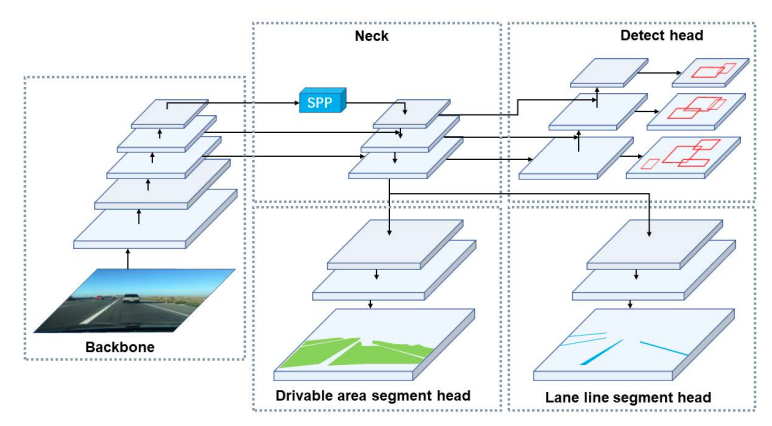
\includegraphics[scale=0.5]{figs/Diseño/YOLOP/yolop-architecture.png}
  \end{center}
  \caption{Arquitectura de YOLOP}
  \label{fig:Arq_YOLOP}
\end{figure}\

YOLOP está compuesto por un codificador para la extracción de características y tres decodificadores para manejar las tareas específicas. Este modelo ha demostrado un rendimiento 
extremadamente bueno en el desafiante conjunto de datos BDD100K\cite{BDD100K}, logrando el estado del arte en las tres tareas en términos de precisión y velocidad. \newline

Nosotros utilizaremos los decodificadores de segmentación del área transitable 
y detención de carriles. El decodificador de segmentación del área transitable utiliza los mapas de características
extraidos por el codificador para realizar una predicción semántica a nivel de pixeles. Esto significa que 
para cada pixel de la imagen, el decodificador de segmentación del área transitable predice si el pixel 
pertenece a un área transitable o no. \newline

El decodificador de detención de carriles, también utiliza los mapas de características extraídos 
por el codificador. Sin embargo, en lugar de predecir si un pixel es transitable o no, este decodificador
predice si un pixel pertenece a un carril de la carretera. \newline
Es importante destacar que estos decodificadores no funcionan de manera aislada, sino que forman parte
de un sistema de aprendizaje multitarea, es decir, se entranaran conjutamente para realizar sus tareas
respectivas, lo que puede mejorar el rendimiento general del sistema.\newline

Ambos decodificadores, deben de recibir una entrada (W/8,H/8,256): \newline 
\begin{enumerate}
  \item \textbf{W/8 y H/8}: Representa la anchura y la altura de la imagen de entrada, respectivamente, divididas por 8.
  \item \textbf{256}: es el número de 
  canales en el tensor de entrada. En el contexto de las redes neuronales convolucionales, 
  un canal puede ser una característica aprendida (como bordes, texturas, colores, etc.) o una capa de color en una imagen (como rojo, verde, azul en imágenes RGB)
\end{enumerate}

Devuelven una salida de tipo (W,H,2), siendo W la anchura y H la altura de la imagen, solo hay dos canales en cada mapa de características, ya que cada píxel 
representa si pertenece a una clase de objeto o al fondo. 

\subsubsection{Modelo de YOLOP}
\label{sec:Modelo_YOLOP}

YOLOP utiliza una arquitectura de red neuronal CNN. Es un tipo de red neuronal artificial diseñada para procesar datos con una
estructura de cuadrícula, como una imagen. Dicho modelo presenta unos pesos preentrenados: 

\begin{enumerate}
  \item \textbf{End-to-end.pth}: Este archivo se ha construido a partir de la biblioteca Pytorch. 
  \item \textbf{Yolop-320-320.onnx, yolop-640-640.onnx y yolop-1020-1020.onnx}: Estos tres archivos se han construido a partir de Onnx.
\end{enumerate}

Dependiendo de que pesos preentrenados queramos utilizar tendremos resultados diferentes en el ámbito de cómputo y rápidez a la hora de 
realizar la inferencia del modelo con los pesos. \newline

\begin{code}[h]
  \begin{lstlisting}[language=Python]
    import torch

    # load model
    model = torch.hub.load('hustvl/yolop', 'yolop', pretrained=True)
    
    #inference
    img = torch.randn(1,3,640,640)
    det_out, da_seg_out,ll_seg_out = model(img)
    
  \end{lstlisting}
  \caption[Cargar modelo YOLOP con pesos preentrenados End-to-end.pth]{Ejemplo básico de cómo poder utilizar YOLOP}
  \label{cod:codejemplo}
  \end{code}  
Este ejemplo se puede encontrar en la página Pytorch dedicada a la red neuronal YOLOP\footnote{\url{https://pytorch.org/hub/hustvl_yolop/}}.

Por lo que, utilizaremos esta red neuronal para poder detectar los carriles que puede tener las áreas transitables en Airsim.

\begin{figure}[H]
  \begin{center}
    \subfigure[Detención de tráfico]{
     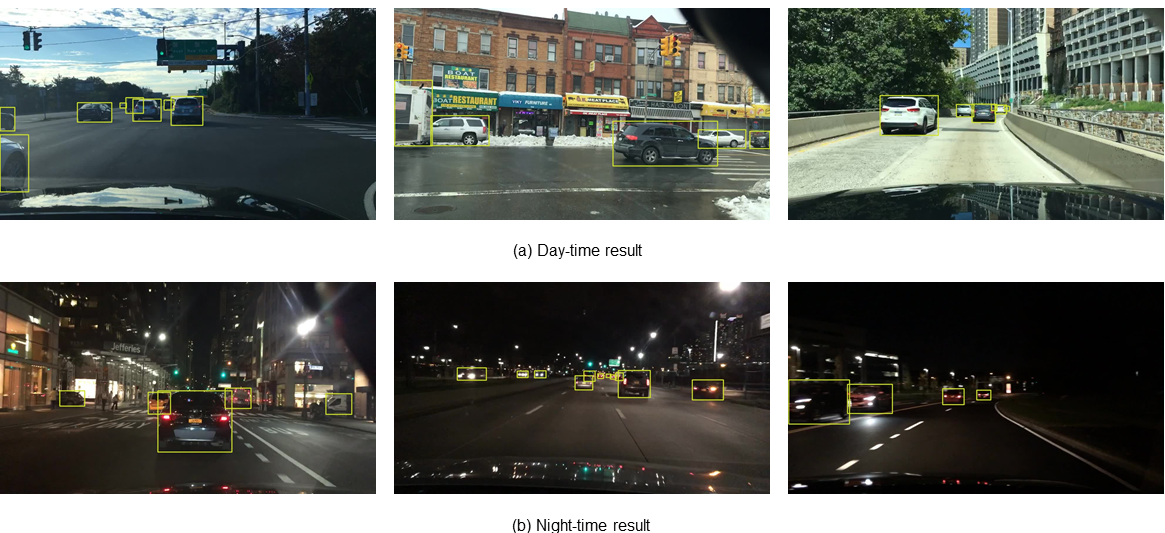
\includegraphics[scale=0.4]{figs/Plataformas_Desarollo/detect.png}
     \label{f:Detención de tráfico}}
    \subfigure[Segmentación de área transitable]{
      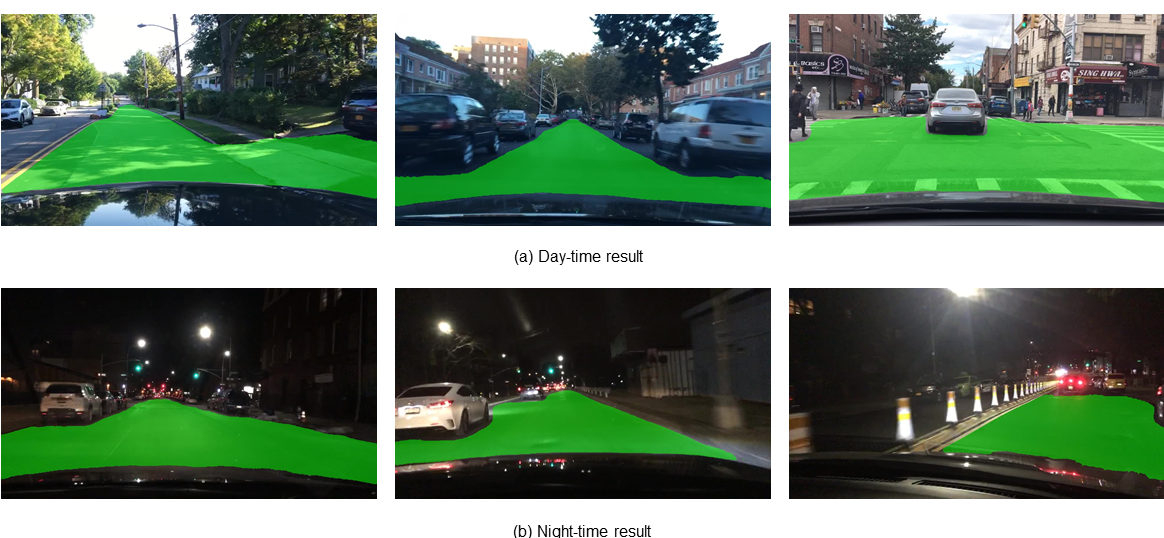
\includegraphics[scale=0.4]{figs/Plataformas_Desarollo/da.png}
      \label{Segmentación}}
    \subfigure[Líneas detectadas]{
      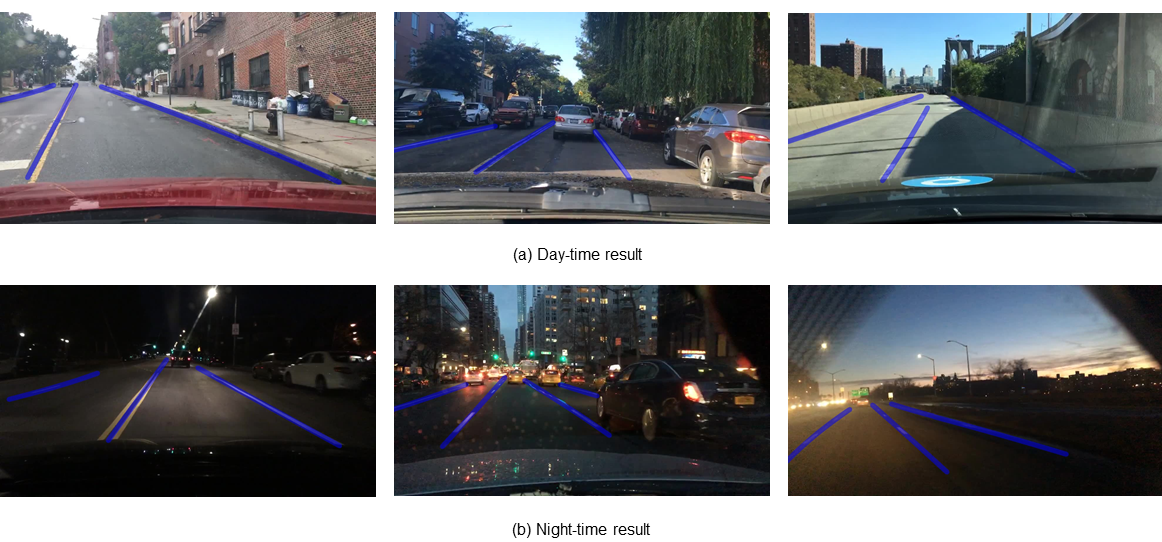
\includegraphics[scale=0.4]{figs/Plataformas_Desarollo/ll.png}
      \label{f:ll}}
  \caption{Resultados de la salida de la red neuronal YOLOP\cite{YOLOP}}
  \label{f:resultadosYOLOP}
  \end{center}
 \end{figure}
 \newpage
\section{ROS}
\label{sec:ros}
\textbf{ROS (Robot Operating System)}\footnote{\url{https://www.ros.org/}} es un conjunto de librerías de código abierto utilizadas principalmente para aplicaciones robóticas. 
Podemos definir este middleware como se muestra en la figura \ref{fig:ROS}:

\begin{figure} [H]
    \begin{center}
      
\includegraphics[scale=0.18]{figs/Plataformas_Desarollo/ros-equation.png}
    \end{center}
    \caption{Definición de ROS}
    \label{fig:ROS}
  \end{figure}\


\begin{enumerate}
    \item \textbf{Plumbing}: ROS proporciona una infraestructura de mensajería publicador-subscriptor diseñada para facilitar la construcción sencilla y rápida de sistemas informáticos
    distribuidos.
    \item \textbf{Tools}: ROS proporciona introspección, lanzamiento, depuración, visualización, trazado, registro, reproducción y detener sistemas informáticos distribuidos.
    \item \textbf{Capabilities}: ROS proporciona una amplia colección de bibliotecas que implementan funciones útiles para los robots, por ejemplo, movilidad, manipulación y percepción.
    \item \textbf{Community}: ROS cuenta con el apoyo y la mejora de una gran comunidad, con un fuerte enfoque en la integración y la documentación, gracias a ello, es una ventaja poder
    aprender a cerca de los miles de paquetes que ofrece ROS que están disponibles de desarrolladores de todo el mundo.
\end{enumerate}

Este middleware sigue un modelo parcialmente centralizado de publicación y suscripción, el cual el publicador genera mensajes y eventos asociados a un topic y el subscriptor
es quien se subscribe al topic correspondiente y recibe la información que ha generado el publicador. \newline

Este tipo sistema es bastante útil ya que permite a los desarrolladores cambiar, añadir o eliminar nodos (programas en ejecución) sin afectar al resto del sistema, facilitando de forma asíncrona
el desarrollo iterativo, permitiendo construir sistemas robóticos complejos, escalables y robustos mejorando la eficiencia y permitiendo el desarrollo y mantenimiento de aplicaciones
robóticas. \newline

Utilizamos ROS en el desarrollo del TFG para realizar la conexión con el simulador Airsim y el desarrollo del sistema de percepción del seguimiento del carril a través del controlador PID y 
aprendizaje por refuerzo. \newline


\begin{figure} [H]
    \begin{center}
      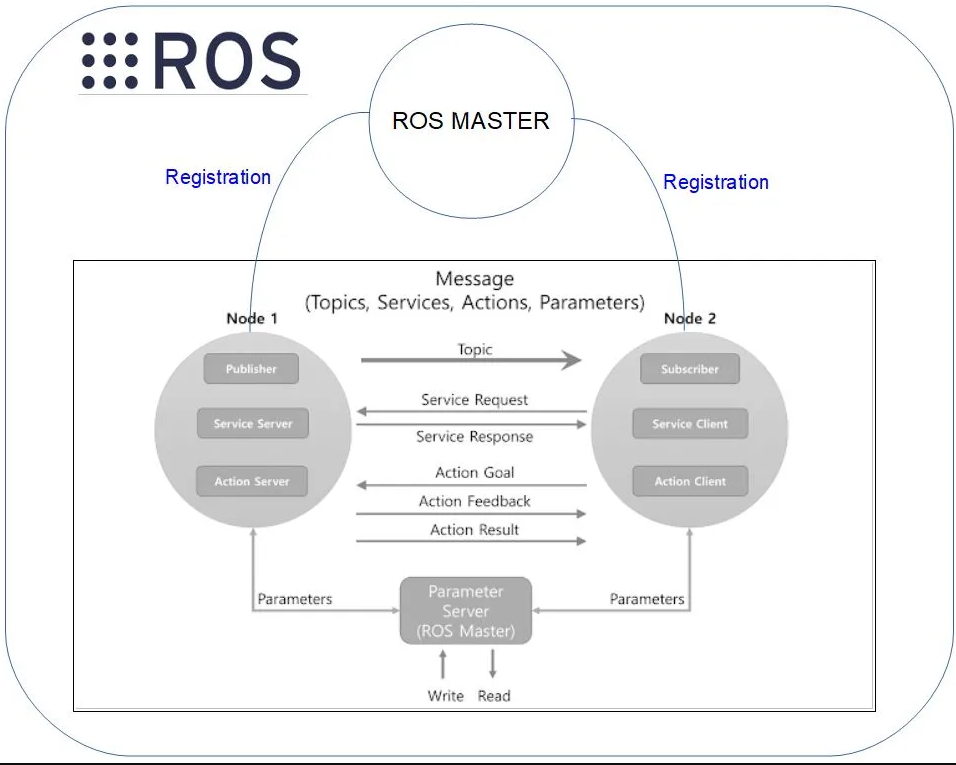
\includegraphics[scale=0.4]{figs/Plataformas_Desarollo/arq_ros.png}
    \end{center}
    \caption{Arquitectura de ROS}
    \label{fig:ArqROS}
  \end{figure}\
\newpage
\subsection{Mavros}
\label{sec:mavros}

\textbf{Mavros}\footnote{\url{http://wiki.ros.org/mavros}} es un paquete formado por \textbf{ROS} y el protocolo de comunicaciones ligero \textbf{MAVLink} (Micro Air Vehicle Link) diseñado por Lorenz Meir\footnote{\url{https://www.technologyreview.es/listas/35-innovadores-con-menos-de-35/2017/inventores/lorenz-meier}} bajo el LGPL licencia. Este protocolo es utilizado para enviar información de estado,
para controlar el vehículo y recibir datos de telemetría. Fácil de implementar en sistemas con recursos limitados, 
lo que lo hace ideal para su uso en drones y otros vehículos aéreos no tripulados. \newline

Ademas, \textbf{Mavros} traduce los mensajes \textbf{ROS} a mensajes \textbf{MAVLink} y viceversa por lo que permite que los datos y comandos fluyan entre \textbf{ROS} y el drone, 
permitiendo un control más sofisticado y una mayor funcionalidad. \newline

Por lo que, en este TFG estudiaremos y analizaremos sí \textbf{Mavros} se podría utilizar para el control del dron junto con \textbf{PX4 AutoPilot} (\ref{sec:px4}) a través
de Airsim. \newline

\begin{figure} [H]
  \begin{center}
    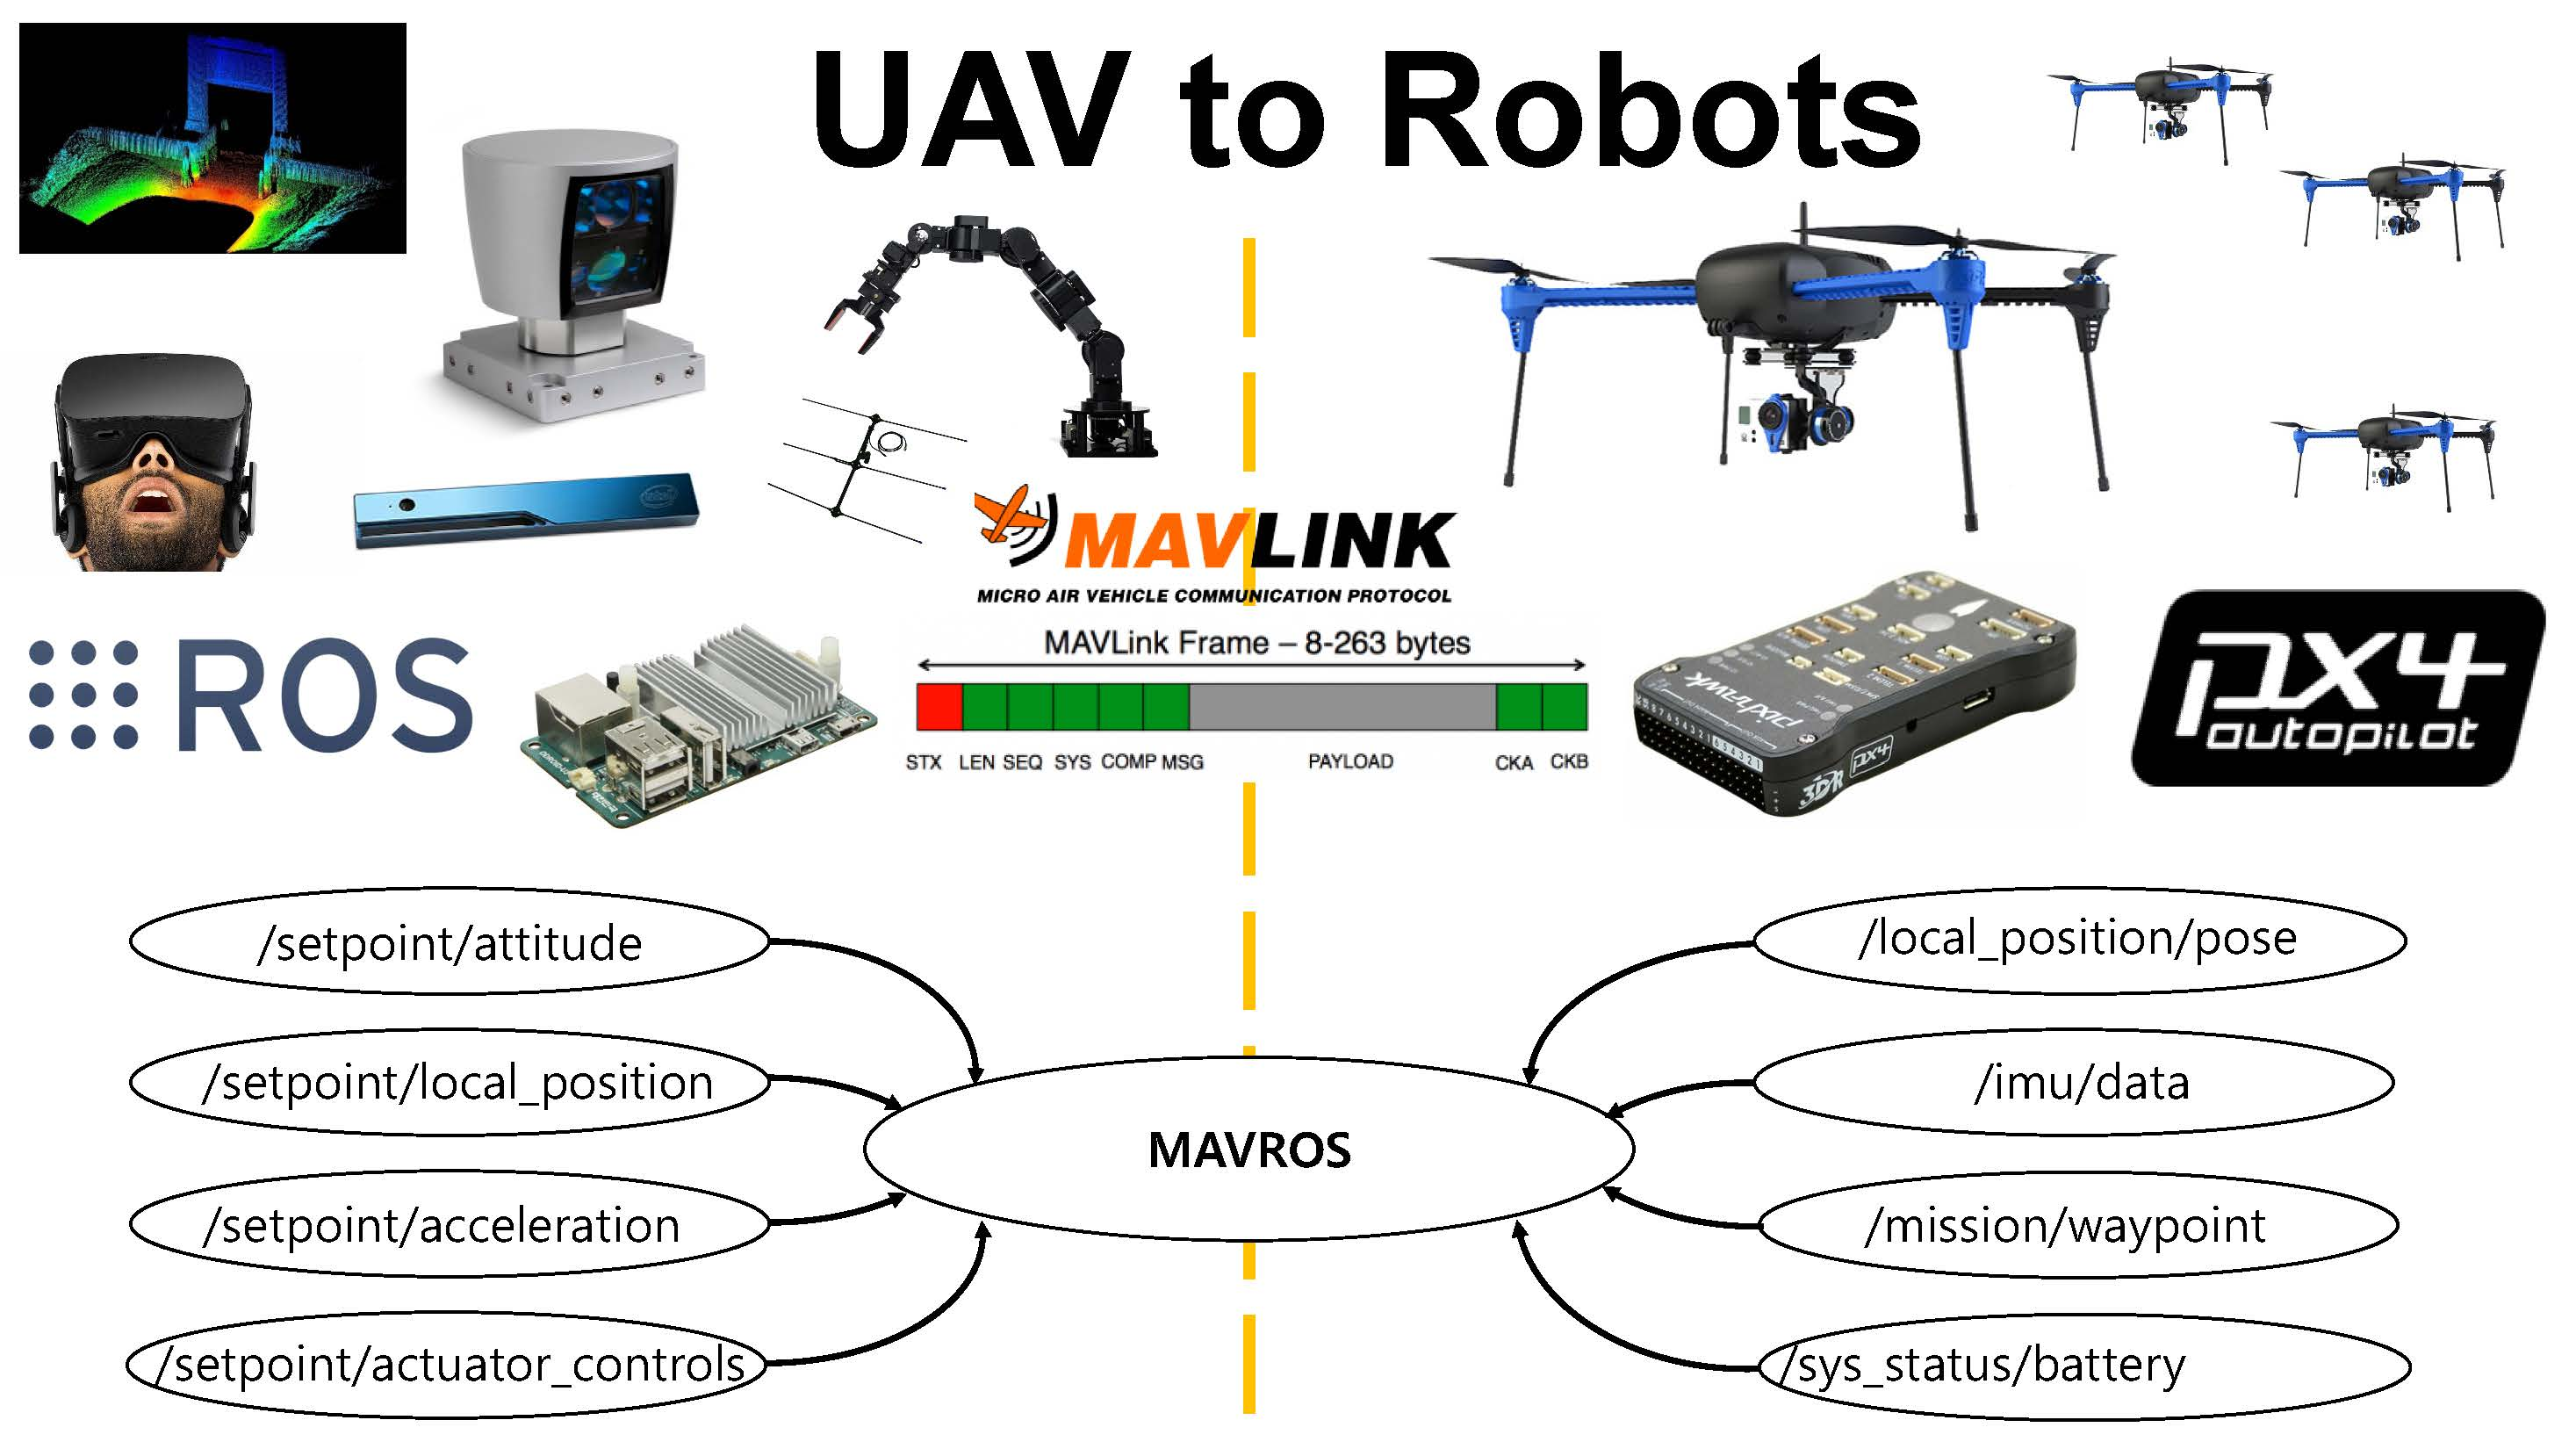
\includegraphics[scale=0.4]{figs/Plataformas_Desarollo/mavros.jpg}
  \end{center}
  \caption{Infraestructura de Mavros}
  \label{fig:InfraROS}
\end{figure}\


\section{Airsim}
\label{sec:Airsim}
El entorno de simulación en el que vamos a estar trabajando será \textbf{Airsim} junto con \textbf{UnRealEngine} de Epic Games\footnote{\url{https://www.unrealengine.com/es-ES}}. \textbf{Airsim}\footnote{\url{https://microsoft.github.io/AirSim/}} es un simulador de código abierto que se utiliza en aplicaciones robóticas 
y aprendizaje automático.
Se construye sobre entornos 3D creados con \textbf{UnRealEngine}, estos entornos son utilizados para simular el mundo real y probar 
cómo los vehículos autónomos se comportarían en diferentes situaciones. \textbf{Airsim} es compatible en varias plataformas como Linux, Windows, macOS y también para Docker y WSL. En nuestro caso,se utilizará en Linux junto
con \textbf{ROS}. \newline

Por otro lado \textbf{UnRealEngine} es un motor de videojuegos que se utiliza para la creación y simulación de entornos 3D realistas para videojuegos,
películas animadas, experiencias interactivas y de realidad virtual. Es una propuesta innovadora utilizar este tipo de herramientas ya que puedes simular 
comportamientos físicos que se puedan producir en un entorno real. \newline

Como hemos comentado anteriormente, \textbf{Airsim} es una buena opción de uso si queremos tener comportamientos
similares a un entorno real. Ofrece una variedad de escenarios, tipos de vehículos, sensores y configuraciones del entorno 
según las necesidades u objetivos marcados de cada persona. 
Para ello se debe todo configurar en un fichero de configuración con extensión json denominado settings.json ,lo cual para configurar
el vehículo con nuestras necesidades necesitaremos definir diferentes variables. \newline

Un archivo settings.json es un archivo de configuración específica de Airsim que define cómo 
se ejecutará la simulación en términos de propiedades del vehículo, configuración de sensores, condiciones climatológicas y más. \newline

Un archivo settings.json consta de varias secciones: 
\begin{enumerate}
  \item \textbf{SimMode}: Este parámetro define el modo de simulación, se refiere si el modo de simulación es para coches, multirotores o vision de computador.
  \item \textbf{ClockType}: Determina qué tipo de reloj se utiliza para medir el tiempo en la simulación. 
  \item \textbf{Vehicles}:Configuración de  las propiedades de cada vehículo individualmente. Puedes especificar el tipo de vehículo, la posición inicial, la dinámica del vehículo, entre otros.
  \begin{itemize}
    \item \textbf{VehicleType}: En este caso ese parámetro es el tipo de vehículo que utilizaremos en la simulación.
    \item \textbf{UseSerial}: Es para saber si vamos a usar un puerto serial en fisico si utilizamos un vehículo en un entorno real.
    \item \textbf{LockStep}: Es una característica importante cuando se comunica con el simulador AirSim a través de TCP.
    \item \textbf{UseTcp}: Para poder comunicarnos a través de TCP necesitamos habilitar esta opción a true.
    \item \textbf{TcpPort}: Especificamos el puerto TCP que vayamos a usar. 
    \item \textbf{ControlIp}: Esta opción es para especificar si el comportamiento se realizará simulado.
    \item \textbf{ControlPortLocal}: Se especificará el puerto Local. 
    \item \textbf{ControlPortRemote}: Se especificará el puerto Remoto.
    \item \textbf{LocalHostIp}: La dirección IP del ordenador en donde llevaremos la simulación.
    \item \textbf{Parameters}: Estos parametros son de PX4 y permite la configuración del vehiculo,
    como por ejemplo los modos de vuelo, sus configuraciones, configuraciones de velocidades y más. 
    \item \textbf{Sensors}: Permite personalizar la configuración de los sensores simulados, como Lidar, IMU (Unidad de Medición Inercial),GPS y sensor de distancia. 
    \item \textbf{Cameras}: Puedes configurar las cámaras utilizadas en la simulación, especificando sus propiedades como resolución, tipo de lente, posición y orientación relativas al vehículo.\newline 
    
    Nosotros usaremos una cámara que proporcionará una imagen RGB de dimensiones 620x620 pixeles y activaremos
    el flag de PublishToRos a 1 para poder acceder a ella mediante el Airsim ROS Wrapper.
  \end{itemize}
\end{enumerate}

Para más detalles sobre el archivo de settings.json está la paǵina oficial de Airsim\footnote{\url{https://microsoft.github.io/AirSim/settings/}} \newline

\subsubsection{Escenarios}
\label{sec:airsim}
Los escenarios que ofrece Airsim depende en que sistema operativo nos encontremos, en nuestro caso al utilizar el escenario en Windows 
tenemos más variedad que en comparación con Linux. \newline

\begin{figure}[H]
  \centering
  \begin{minipage}{0.5\textwidth}
      \centering
      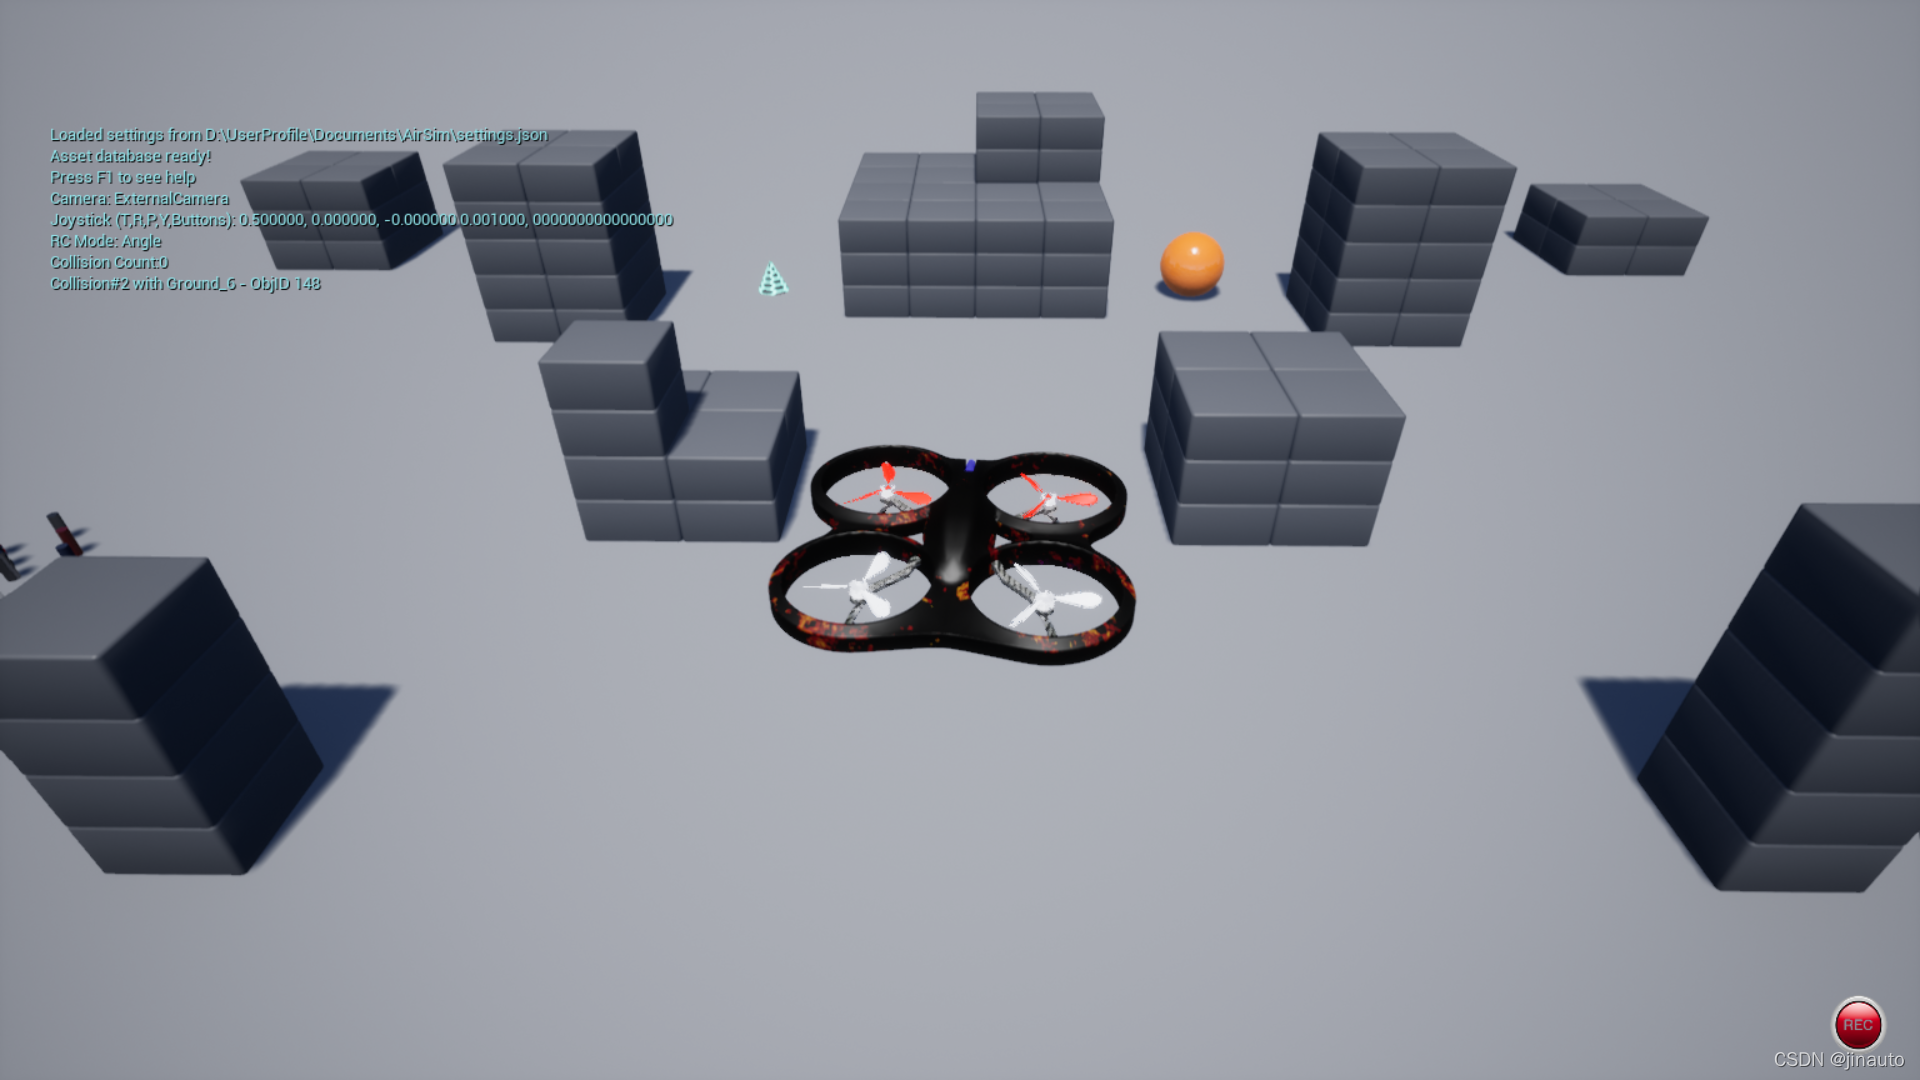
\includegraphics[width=\linewidth]{figs/Plataformas_Desarollo/mapas_airsim/blocks.png}
      \caption*{a) Blocks}
  \end{minipage}%
  \begin{minipage}{0.5\textwidth}
      \centering
      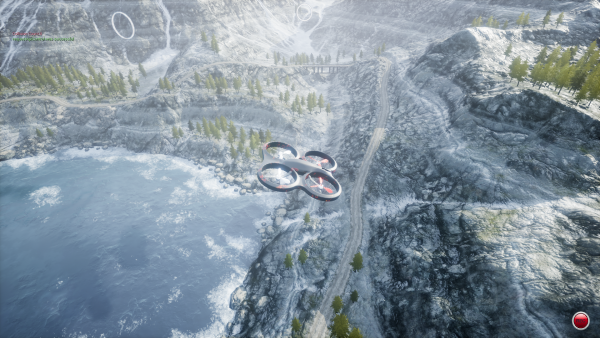
\includegraphics[width=\linewidth]{figs/Plataformas_Desarollo/mapas_airsim/landscapemountains.png}
      \caption*{b) LandscapeMountains}
  \end{minipage}

  \begin{minipage}{0.5\textwidth}
      \centering
      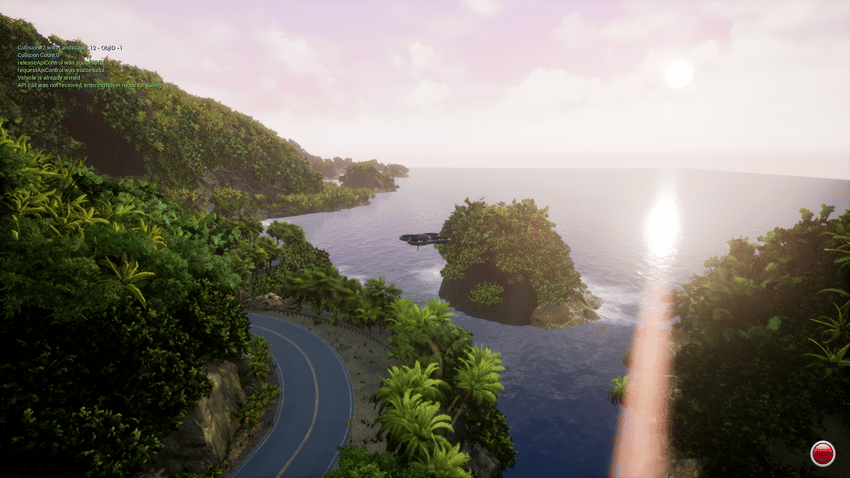
\includegraphics[width=\linewidth]{figs/Plataformas_Desarollo/mapas_airsim/Coastline.png}
      \caption*{c) Coastline}
  \end{minipage}%
  \begin{minipage}{0.5\textwidth}
      \centering
      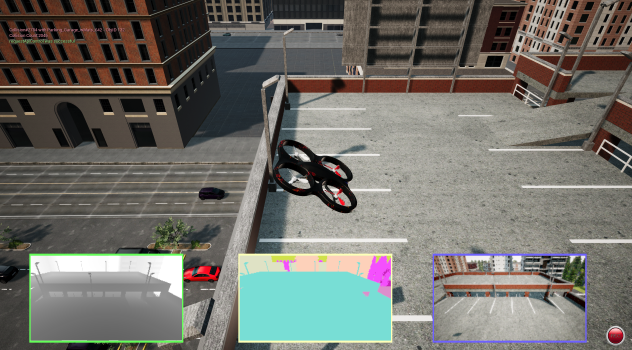
\includegraphics[width=\linewidth]{figs/Plataformas_Desarollo/mapas_airsim/city_airsim.png}
      \caption*{d) City}
  \end{minipage}

  \begin{minipage}{0.5\textwidth}
      \centering
      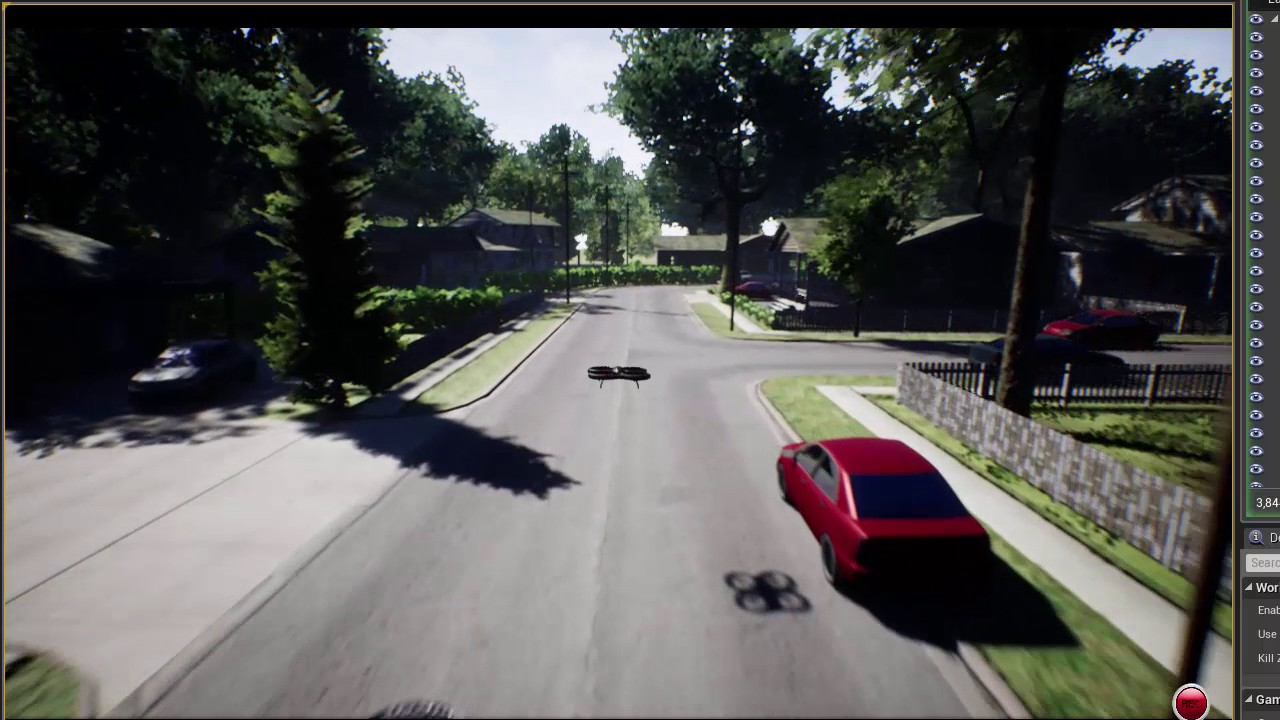
\includegraphics[width=\linewidth]{figs/Plataformas_Desarollo/mapas_airsim/AirsimNH.jpg}
      \caption*{e) Neighborhood}
  \end{minipage}
  \caption{Ejemplos de escenarios en Airsim}
  \label{f:escenarios_airsim}
\end{figure}

Tiene escenarios desde carreteras y cuidades con coches simulados hasta entornos industriales como almacenes y entornos de montaña con carreteras como se 
muestra en la figura \ref{f:escenarios_airsim}. En nuestro caso
hemos utilizado el escenario Coastline,consiste en un entorno fotorrealista de un recorrido amplio de 2 carriles con ambiente tropical. Con este entorno tendremos la
información del entorno para realizar el comportamiento sigue carril con el dron. \newline

Todos estos escenarios se pueden encontrar en las releases de Airsim\footnote{\url{https://github.com/Microsoft/AirSim/releases}} tanto para Windows como para Linux.
En nuestro caso hemos utilizado el escenario Coastline, ya que queremos desarrollar un comportamiento de seguimiento de carril y este escenario ofrece un amplio recorrido de 2 carriles para poder llevarlo
a cabo.



\subsubsection{Sensores}
\label{sec:airsim}
Ofrece sensores como cámaras, barómetros, Imus, GPS, Magnetómetros, sensores de distancia y Lidar.
En nuestro caso utilizaremos como sensores una cámara para poder realizar la detención del carril 
que queremos seguir, el sensor Lidar para saber a que altura se encuentra el dron respecto al suelo y el sensor
GPS para poder obtener la localización del vehículo. 

\subsubsection{Tipos de vehículos}
\label{sec:airsim}
\textbf{Airsim} ofrece dos tipos principales de vehículos para la simulación: coches y drones. Dentro de estos tipos se encuentran los subtipos de coches y drones que se puede utilizar.

\begin{enumerate}
  \item \textbf{Coche}
    \begin{itemize}
      \item \textbf{PhysXCar}: Representa un vehículo en tierra con física realista basado en el motor de física PhysX.
      \item \textbf{ArduRover}: Se utiliza para vehículos terrestres que sigan el estándar ArduRover. ArduRover\footnote{\url{https://ardupilot.org/rover/}} 
      se trata de un piloto automático de código abierto utilizado especificamente para vehículos terrestres.
      \newline
    \end{itemize}
    
  \item \textbf{Dron}
    \begin{itemize}
      \item \textbf{SimpleFlight}: Representa un dron con un modelo de vuelo simplificado. Este tipo de opción puede ser útil si queremos simular comportamientos 
      de movimiento básico para los drones.
      \item \textbf{PX4Multirotor}: Representa un dron mediante PX4 ArduPilot. 
      \item \textbf{ArduCopter}: Representa un dron pero siguiendo el estándar ArduCopter. ArduCopter\footnote{\url{https://ardupilot.org/copter/}} 
      se trata de un piloto automático de código abierto utilizado para los drones 
    \end{itemize}
  
\end{enumerate}

Como hemos numerado anteriormente, este entorno de simulación tiene un catálogo de vehículos, sensores y
cambios climatológicos dentro del entorno. Nosotros utilizaremos un dron de tipo "SimpleFligh". 

\subsection{Airsim ROS Wrapper}
\label{sec:wrapper}
Utilizaremos el paquete \textbf{Airsim ROS Wrapper}\footnote{\url{https://microsoft.github.io/AirSim/airsim_ros_pkgs/}} para poder acceder a ciertos sensores 
que serán necesarios como es la cámara,el Lidar y el GPS, pero antes de comentar lo que ofrece hablaremos sobre que es un ROS Wrapper. \newline

\textbf{ROS Wrapper} es un componente que facilita la integración entre dos sistemas o entornos diferentes. Si lo llevamos al contexto de \textbf{ROS}, un wrapper es un nodo o paquete 
que permite que los componentes de \textbf{ROS} se comuniquen con otros sistemas o bibliotecas que no fueron originalmente diseñadas para trabajar con \textbf{ROS}. Este paquete 
puede proporcionar publicación de datos desde el sistema externo a \textbf{ROS} a través de topics, suscripción a topics de \textbf{ROS} para recibir comando o datos, adaptación 
de interfaces de llamada (por ejemplo, entre C++ y Python). \newline

Por lo tanto, \textbf{Airsim ROS Wrapper} es un paquete de \textbf{ROS} que comunicará \textbf{ROS} y \textbf{Airsim}. Este paquete contiene dos nodos principales 
que han sido realizados mediante la comunidad de Airsim\footnote{\url{https://github.com/microsoft/AirSim}}:
\begin{enumerate}
  \item \textbf{AirSim ROS Wrapper Node}: Este nodo proporciona una interfaz \textbf{ROS} para acceder a los datos del vehículo simulado, por ejemplo, sus sensores, proporcionar velocidades, acceder a su sistema de referencia,etc. 
  \item \textbf{Simple PID Position Controller Node}: Este nodo es un controlador de posición simple basado en un controlador PID (proporcional-derivativo-integral). Ayuda controlar la posición del vehículo 
  simulado en el entorno \textbf{Airsim}.
\end{enumerate}

\subsection{Client Airsim}
\label{sec:Client Airsim}

Airsim ofrece una API implementada para Python demoninada Client Airsim\footnote{\url{https://microsoft.github.io/AirSim/apis/}}, en donde podemos conectarnos con el simulador y tener el control de los sensores y actuadores del vehículo. 
Esta interfaz es bastante útil ya que podemos tener el control del vehículo simulado sin necesidad de tener que utilizar los topics de ROS, es decir, existen métodos los cuales
podemos comandar velocidades al vehículo, tener acceso a los sensores como las cámaras o cambiar configuraciones de la simulación como por ejemplo el clima, el viento, el tiempo del día
o la densidad de tráfico en escenarios donde aparecen coches simulados. \newline

Esta API la utilizaremos sobre todo para tener el control del vehículo para realizar su navegación con los controladores PID y en 
el desarrollo de aprendizaje por refuerzo. 

\section{PX4 AutoPilot}
\label{sec:px4}

\textbf{PX4}\footnote{\url{https://docs.px4.io/main/en/}} es una plataforma de software de código abierto para desarrolladores de drones que les permite crear 
y controlar diversos tipos de drones,desde aplicaciones de consumo hasta aplicaciones industriales. \newline

Unas de las principales características que ofrece esta plataforma es el soporte de múltiples tipos de vehículos, como aviones de 
ala fija, multirrotores, helicópteros, rovers y vehículos submarinos, también proporciona diferentes modos de vuelo, 
navegación por puntos de referencias predefinidos, estabilización del vehículo. \newline

En este trabajo realizaremos un analisis respecto a la navegación del dron mediante \textbf{PX4} con el modo de simulación Software in The Loop(SITL) para tener el control el vehículo junto con 
\textbf{Mavros} y \textbf{Airsim}.\newline
\subsection{Software in The Loop(SITL)}
\label{sec:px4 sitl} 
Este modo de simulación permite a los desarrolladores probar y depurar códigos de control de drones sin necesidad de hardware físico, en lugar de ejecutar el código en un 
vehículo real, este modo simula el comportamiento del vehículo en una computadora. Es especialmente útil durante el desarrollo y la validación de control, navegación y 
planificación de misiones. \newline

Podemos tener diversos entornos de simulación con este modo como Gazebo, Airsim y jMAVSim. Dichos entornos de simulación permiten realizar simulaciones muy realistas y avanzadas 
de cualquier tipo de vehículo simulando una gran variedad de parámetros.\newline

Para poder utilizar PX4 SITL, se debe configurar el entorno de desarrollo adecuado y seguir las instrucciones proporcionadas por la comunidad\footnote{\url{https://docs.px4.io/v1.14/en/simulation/}} .
En nuestro caso realizaremos la configuración PX4 SITL junto con Airsim para estudiar si es posible tener un control en el comportamiento a querer
desarrollar. 

\subsection{Modos de vuelo}
\label{sec:flight modes} 

PX4 ofrece varios modos de vuelo por ejemplo como Takeoff,Land,Hold, Position, Offboard, etc. Un modo de vuelo define como el usuario puede controlar el vehículo a través de comandos
  y ver que respuesta tiene. 


  \begin{enumerate}
    \item \textbf{TAKEOFF}: Este modo de vuelo permite despegar el vehículo con una altitud y una velocidad de ascendiente escogida por el usuario con los parametros de PX4 MIS\_TAKEOFF\_ALT y
    MPC\_TKO\_SPEED, dichos parametros tienen valores por defectos definidos por la plataforma (2.5 m y 1.5 m/s respectivamente). Antes de realizar el despegue el vehículo sera armado 
    para poder realizarlo.

    Una vez se realice el despegue del vehículo se pasa al modo HOLD 
    \item \textbf{LAND}: Permite aterrizar el vehiculo en donde nos encontremos en ese instante, una vez el vehículo sea aterrizado se desarmará por defecto. En este modo podemos cambiar por ejemplo
    la tasa de descenso durante se realiza el aterrizaje del vehículo con el parametro MPC\_LAND\_SPEED, tiempo en segundos para que se realice el desamardo del vehículo si se establece dicho tiempo
    con un valor de -1 el vehículo no se desarmará cuando aterrice.
    
    Cuando de realice este modo de vuelo por defecto se cambiará al modo de Position

    \item \textbf{HOLD}: A partir de este modo de vuelo podemos parar el vehículo manteniendolo en el aire con su actual posición GPS y altitud. Este modo puede ser bastante útil para cuando queremos
    pausar una mision o reiniciar el comportamiento que queramos realizar. 

    \item \textbf{POSITION}: Es un modo de vuelo manual el cual puedes controlar el vehículo mediante un joystick, dicho vuelo controla la posición del vehículo cuando comandemos velocidades 
    mediante el joystick. Este modo de vuelo lo utilizaremos para teleoperar el dron para ver el funcionamiento de la percepción por parte de la red neuronal que utilizaremos.
    Dicho vuelo ofrece un gran catalogo de parametros que puede afectar al vuelo.

    \begin{figure} [H]
      \begin{center}
        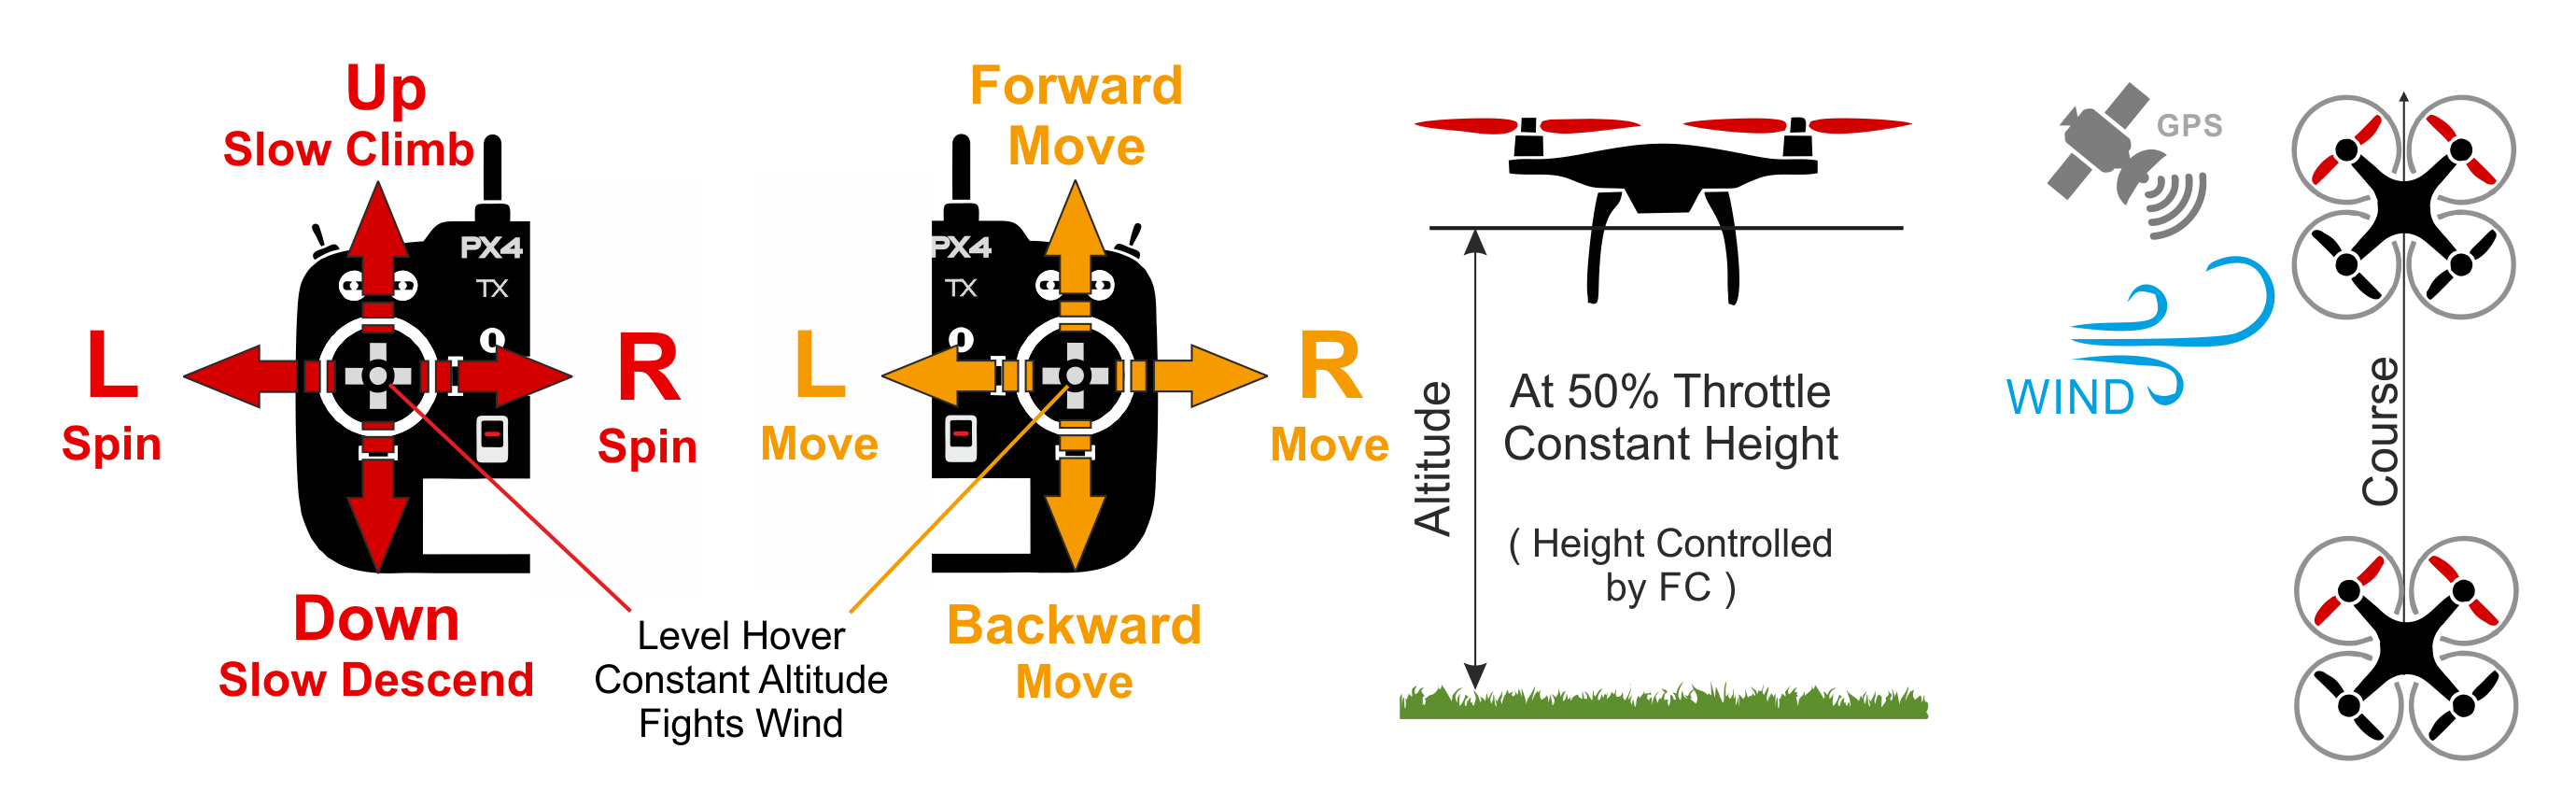
\includegraphics[scale=0.6]{figs/Diseño/PX4/position_MC.png}
      \end{center}
      \caption{Diagrama del comportamiento del modo de vuelo Position}
      \label{fig:position_mode_px4}
    \end{figure}\

    \item \textbf{OFFBOARD}: Con este modo de vuelo podemos controlar el movimiento y la altitud del vehículo a partir de comandos de posición, velocidad, aceleración, altitud, velocidades de 
    altitud o puntos de ajuste de empuje/torque. 

    Dichos comandos debe ser una secuencia de mensajes de setpoint MavLink o a través de topics mediante ROS con Mavros.

    En este modo,PX4 debe recibir una secuencia de mensajes continua. Si en algún momento dejamos de publicar mensajes, el control externo de PX4 dejará de estar en el modo Offboard después
    de pasar un tiempo de espera establecido por el parámetro COM\_OF\_LOOS\_T (por defecto esta establecido a 1 s) e intentará aterrizar o realizar alguna acción de seguridad (dichas acciones 
    de seguridad vienen definidas en la seccion de Failsafes en PX4 Autopilot\footnote{\url{https://docs.px4.io/v1.14/en/config/safety.html}}). La acción dependerá
    si el control RC está disponible, si este control esta disponible pasará a otro tipo de modo de vuelo definido en el parámetro COM\_OBL\_RC\_ACT. 

    Para comandar las velocidades al vehículo mediante Mavros, se tendrá que utilizar el topic denominado /mavros/setpoint\_velocity/cmd\_vel\_unstamped dicho topic utiliza el un marco de coordenadas
    por defecto definido en el archivo de configuración de px4.config.yaml  LOCAL\_NED. Si queremos que el marco de coordenadas se mueva con el 
    cuerpo del vehiculo se tendrá que utilizar el marco de coordenadas
    En nuestro caso necesitamos un marco de coordenadas diferente para que el vehiculo se mueva
    con el cuerpo del vehículo, por ello utilizaremos el marco de coordenadas BODY\_NED. 

    Los marcos de coordenadas que ofrece Mavros se puede ver a través del servicio SetMavFrame.srv\footnote{\url{https://github.com/mavlink/mavros/blob/master/mavros_msgs/srv/SetMavFrame.srv}}
  \end{enumerate}

\section{QGroundControl}
\label{sec:QGroundControl} 

\textbf{QGroundControl}\footnote{\url{http://qgroundcontrol.com}} es una plataforma de software que proporciona un control completo de vuelo 
y configuraciones de vehículos para drones por \textbf{PX4 ArduPilot}. Además, ofrece un control total durante el vuelo y permite la planificación de vuelos autónomos 
mediante la definición de puntos de referencia, se muestra la posición del vehículo junto con su trayectoria, los puntos de referencia y los instrumentos del vehículo. 
Es una opción cómoda para poder visualizar tu vehículo y querer cambiar parámetros del vehículo mediante esta aplicación y poder teleoperar el vehículo a través de un mando joystick. \newline

Funciona en diferentes plataformas como Windows, macOS, Linux,iOS y dispositivos Android, en nuestro caso lo utilizaremos en Linux. 

\begin{figure} [h]
  \begin{center}
    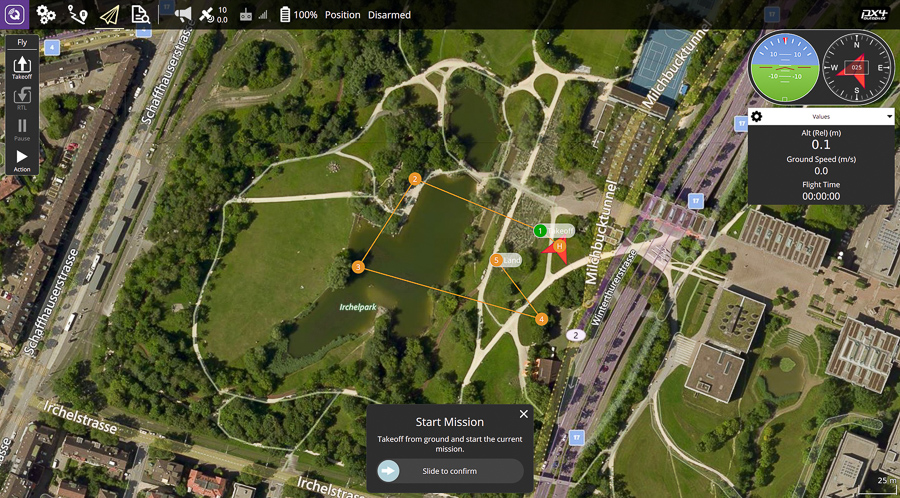
\includegraphics[scale=1.2]{figs/Plataformas_Desarollo/software-qgc.jpg}
  \end{center}
  \caption{QGroundControl}
  \label{fig:QGroundControl}
\end{figure}\



































%\input{capitulos/Diseño}
\chapter{Anexo}
\label{cap:anexo}
\setcounter{page}{1}
A continuación se muestra las diferentes referencias a las figuras que hemos visto a lo largo de este trabajo junto con el enlace 
de donde ha sido obtenida. Las imagenes que no incluidas en este capítulo han sido formadas en el desarollo de este trabajo provienen 
del mismo: 

\begin{tabular}{ | m{4cm} | m{10cm}| m{1cm} | }
    \hline
    \textbf{Referencia de las imágenes} & \textbf{Enlaces de donde se ha obtenido}  \\
    \hline
    \ref{fig:Sojourner} & \url{https://airandspace.si.edu/multimedia-gallery/web12070-2011640jpg} \\ 
    \hline
    \ref{fig:Nereus} & \url{https://www.whoi.edu/oceanrobots/robots/nereus-phone.html} \\ 
    \hline
    \ref{fig:Agrobot} & \url{https://www.diariosur.es/economia/agroalimentacion/salado-digitalizacion-campo-20201103180516-nt.html} \\
    \hline
    \ref{f:Drones} & \url{https://www.smithsonianmag.com/arts-culture/unmanned-drones-have-been-around-since-world-war-i-16055939/} \newline
    \url{https://web.happystays.com/?m=file-winston-churchill-and-the-secretary-of-state-for-tt-YQ3jGVI4} \newline
    \url{https://en.wikipedia.org/wiki/V-1_flying_bomb} \newline  
    \url{https://www.google.com/url?sa=i&url=https%3A%2F%2Fthefrontlines.com%2Fstory%2Fww2-project-aphrodite%2F&psig=AOvVaw2OcBlgMDHlHVU5qsiJ9_Fg&ust=1714151925046000&source=images&cd=vfe&opi=89978449&ved=0CBQQjhxqFwoTCNjGs9bv3YUDFQAAAAAdAAAAABAE} \newline
    \url{https://en.wikipedia.org/wiki/Ryan_Firebee} \newline
    \url{https://en.wikipedia.org/wiki/Lockheed_D-21} \newline
    \url{https://www.google.com/url?sa=i&url=https%3A%2F%2Fwww.researchgate.net%2Ffigure%2FBoeing-Condor-UAV-23_fig10_261209014&psig=AOvVaw1q3J6eh2YCyEUzy1QM9z_K&ust=1714152091161000&source=images&cd=vfe&opi=89978449&ved=0CBQQjhxqFwoTCJDAyqXw3YUDFQAAAAAdAAAAABAE} \newline
    \url{https://www.timesofisrael.com/idf-launches-probe-after-two-more-mini-drones-crash/} \newline
    \url{https://www.google.com/url?sa=i&url=https%3A%2F%2Fnews.usni.org%2F2020%2F09%2F15%2Fmarines-placing-small-uavs-into-ground-combat-element-as-aviators-still-refining-large-uas-requirement&psig=AOvVaw2csv7vma6UxJokGvlG8j7h&ust=1714152048517000&source=images&cd=vfe&opi=89978449&ved=0CBQQjhxqFwoTCLiCtZHw3YUDFQAAAAAdAAAAABAE} \\
    \hline 
    \ref{fig:Ingenuity} & \url{https://www.xataka.com/espacio/helicoptero-ingenuity-ha-aterrizado-lugares-marte-que-nasa-se-esta-quedando-letras-para-nombrarlos} \\
    \hline
   
   
   
\end{tabular}

\begin{tabular}{ | m{4cm} | m{10cm}| m{1cm} | }

    \hline 
    \ref{fig:Fenosa} & \url{https://www.elcorreogallego.es/hemeroteca/union-fenosa-distribucion-implanta-uso-drones-supervisar-sus-lineas-alta-tension-galicia-MQCG1024080} \\
    \hline
    \ref{fig:PrimerPrimeAir} & \url{https://www.xataka.com/drones/asi-es-el-dron-repartidor-de-amazon-todavia-poco-mas-que-humo-que-promete-entregar-paquetes-en-media-hora} \\ 
    \hline
    \ref{fig:MK27-2} & \url{https://www.techtimes.com/articles/285562/20221228/amazon-begins-prime-air-drone-deliveries-california-texas.htm} \\
    \hline
    \ref{fig:MK30} & \url{https://emprendedores.es/marketing-y-ventas/ecommerce-marketing-y-ventas/drones-amazon-europa/} \\
    \hline
    \ref{fig:Efficient} & \url{https://www.researchgate.net/publication/273392596_Efficient_Road_Detection_and_Tracking_for_Unmanned_Aerial_Vehicle} \\
    \hline
    \ref{fig:DronesFuturo} & \url{https://aceroestudio.com/drones-en-la-infraestructura-estado-del-arte-y-perspectivas-de-futuro/} \\
    \hline
    \ref{fig:ClasificaciónIA} & \url{https://www.researchgate.net/publication/378676909_The_prospect_of_artificial_intelligence_to_personalize_assisted_reproductive_technology} \\
    \hline
    \ref{fig:Reinforcement Learning} & \url{https://becominghuman.ai/the-very-basics-of-reinforcement-learning-154f28a79071} \\
    \hline
    \ref{fig:Espiral} & \url{https://www.lifeder.com/modelo-espiral/} \\
    \hline 
    \ref{fig:github} & \url{https://github.com/RoboticsLabURJC/2022-tfg-barbara-villalba/graphs/contributors} \\
    \hline  



\end{tabular}



\begin{tabular}{ | m{4cm} | m{10cm}| m{1cm} | }

    \hline
    \ref{fig:Arq_YOLOP} & \url{https://pytorch.org/hub/hustvl_yolop/} \\
    \hline
    \ref{fig:ROS} & \url{https://www.ros.org/imgs/ros-equation.png} \\
    \hline
    \ref{fig:ArqROS} & \url{https://medium.com/@robtech.impaciente/ros-robot-operating-system-fundamentos-e92478c26e02} \\
    \hline
    \ref{fig:InfraROS} & \url{https://404warehouse.net/2015/12/20/autopilot-offboard-control-using-mavros-package-on-ros/} \\
    \hline
    \ref{f:escenarios_airsim} & \url{https://img-blog.csdnimg.cn/272026cef41047cdb7e523fb9a28e173.png?x-oss-process=image/watermark,type_d3F5LXplbmhlaQ,shadow_50,text_Q1NETiBAamluYXV0bw==,size_20,color_FFFFFF,t_70,g_se,x_16} \newline
    \url{https://www.scrimmagesim.org/sphinx/html/_images/Asset_LandscapeMountains_1.png} \newline
    \url{https://www.researchgate.net/figure/Appearance-of-the-maps-for-training-a-City-environment-b-Coastline-c_fig7_359436337} \newline
    \url{https://www.scrimmagesim.org/sphinx/html/_images/city_airsim_view.png} \newline
    \url{https://github.com/Microsoft/AirSim/wiki/moveOnPath-demo} \\
    \hline
    \ref{fig:position_mode_px4} & \url{https://docs.px4.io/v1.14/en/flight_modes_mc/position.html} \\
    \hline
    \ref{fig:QGroundControl} & \url{https://flathub.org/es/apps/org.mavlink.qgroundcontrol} \\
    \hline

\end{tabular}









%\chapter{Conclusiones}
\label{cap:capitulo5}

En este TFG se han cumplido los objetivos marcados durante el desarrollo de él mismo. Primero la creación de algoritmos de
navegación autónoma para drones para resolver la problemática de seguimiento de carril en entornos de carreteras
urbanas. En segundo lugar la utilización de algoritmos basados en inteligencia artificial y aprendizaje no supervisado
con el fin de evaluar su efectividad. Tercero, analizar el desarrollo de aplicaciones de navegación autónoma drones
utilizando el simulador fotorrealista Airsim junto con el middleware robóticos ROS empleando una arquitectura de
comunicación distribuida. 

En conclusión, se comenta los objetivos que se han cumplido a lo largo del desarrollo como los requisitos cumplidos
que se expusieron en el capítulo 2, englobando líneas futuras dentro del trabajo. 

\section{Objetivos cumplidos}
\label{objetivos_cumplidos}

Los objetivos presentados en la sección \ref{sec:descripcion}, han sido cumplidos exitosamente 
\begin{enumerate}
    \item Se logró la instalación y configuración del simulador Airsim junto con ROS, estableciendo la comunicación efectiva
    entre dos equipos mediante protocolos de red. 
    \item Se implementó satisfactoriamente una aplicación de seguimiento de carril utilizando dos tipos de comportamientos,
    el comportamiento clásico mediante un controlador PID y el comportamiento mediante aprendizaje por refuerzo. Utilizando
    en ambos redes neuronales, algoritmos de aprendizaje no supervisado en el sistema perceptivo. 
    \item Se completó de manera exitosa los análisis de los diferentes modelos que nos puede ofrecer la red neuronal YOLOP,
    realizado. 
    \item Se han completado análisis efectivos para cada uno de los comportamientos desarrollados contrastando sus métricas
    de forma exitosa tanto en el sistema perceptivo como de control. 
\end{enumerate}

\section{Requisitos satisfechos}
\label{requisitos_satisfechos}

En la sección \ref{sec:requisitos} se presentaron los requisitos que ha tenido este TFG, que se han ido resolviendo 
de la siguiente forma: 

\begin{enumerate}
    \item Durante todo el proceso del trabajo se utiliza Airsim junto con UnrealEngine como entorno de simulador.
    \item Los comportamientos desarrollados durante el trabajo se ha utilizado la estructura de ROS junto con la comunicación
    del entorno de simulación Airsim. 
    \item La navegación autónoma basada en aprendizaje por refuerzo ha demostrado ser lo suficiente robusta y eficiente en los
    diferentes trayectos dentro del escenario Coastline. 
    \item Uso del algoritmo de Q-Learning para desarrollar el comportamiento sigue carril y de carreteras basados en aprendizaje por 
    refuerzo.
\end{enumerate}


\section{Balance global y competencias adquiridas}
\label{balance_global_competencias_adquiridas}
Durante el desarrollo de este TFG, el desafío de implementar una aplicación de navegación autónoma de drones basada en
aprendizaje por refuerzo y uso de redes neuronales resultó ser un proceso complejo y enriquecedor. Además de que la
combinación de aprendizaje por refuerzo e inteligencia artificial es una estrategia viable y efectiva para la
navegación autónoma de drones. Los resultados obtenidos son prometedores y sugieren que, con más investigación y
desarrollo, estos sistemas pueden ofrecer soluciones robustas y eficientes para la navegación autónoma en una variedad
de entornos sumando la arquitectura de conexión que se llego a implementar para ello. 

Al comienzo de este trabajo apenas tenía suficientes conocimientos básicos sobre inteligencia artificial enfocada en
redes neuronales y aprendizaje por refuerzo. Destacando que ha sido mi primer trabajo de investigación en donde he
aprendido múltiples conceptos, así como adquirir técnicas de análisis de errores que han ido apareciendo durante todo
el proceso. Destacando las siguientes competencias: 

\begin{itemize}
    \item Organización en cuanto a tiempos y tareas utilizando la metodología Kanban.
    \item Nuevos conocimientos en la utilización de simuladores robóticos.
    \item Nuevos conocimientos dentro del área de inteligencia artificial, así como redes neuronales y algoritmos de
    aprendizaje no supervisado. 
    \item Nuevos conocimientos desde cero sobre comportamientos basados en aprendizaje por refuerzo.
    \item Capacidad de analizar diferentes resultados recogidos en los diferentes comportamientos implementados.
    \item Mejora en la capacidad de implementar una arquitectura distribuida entre ambos equipos.
    \item Nuevos conocimientos sobre la integración de ROS junto con aplicaciones externas.
    \item Capacidad de documentación a la hora de desarrollar los diferentes comportamientos. 
\end{itemize}

\section{Líneas futuras}
\label{lineas_futuras}
Aunque hemos obtenido resultados exitosos y satisfactorios a lo largo del TFG, existen diferentes líneas futuras que se
podrían desarrollar a partir de este trabajo. \newline

\begin{itemize}
\item Utilizar la red neuronal usada en el trabajo y volver a entrenar dicha red en el entorno de trabajo teniendo en
cuenta la visión de un dron.
\item Exploración de otras técnicas de algoritmos de clasificación para poder obtener mejores resultados en cuanto a
clasificación.
\item Búsqueda sobre la infraestructura que existe entre el simulador PX4 Autopilot y Airsim, para tener mejores
comportamientos en cuanto a rendimiento y latencia.
\item Mejorar los sistemas de seguimiento de carril de aprendizaje por refuerzo sin las propias limitaciones que puede
presentar el algoritmo de Q-learning.
\item Probar el TFG en diferentes escenarios distintos, con circuitos con curvas más cerradas, con situaciones de tiempo
adversas. 
\end{itemize}

\clearpage
\thispagestyle{empty}

\printindex \nocite{*}
\appendix
\bibliographystyle{apalike} \bibliography{bibliografia}

\end{document}
